\documentclass[11pt,a4paper]{article}
\usepackage[utf8]{inputenc}
\usepackage[T1]{fontenc}
\usepackage{geometry}
\usepackage{graphicx}
\usepackage{hyperref}
\usepackage{amsmath}
\usepackage{amssymb}
\usepackage{booktabs}
\usepackage{xcolor}
\usepackage{fancyhdr}
\usepackage{titlesec}
\usepackage{enumitem}
\usepackage{tcolorbox}
\usepackage{tikz}
\usepackage{pgfplots}
\pgfplotsset{compat=1.18}

\geometry{margin=1in}
\hypersetup{
    colorlinks=true,
    linkcolor=persianblue,
    filecolor=magenta,
    urlcolor=cyan,
    pdftitle={CYRUS Whitepaper - Token of the Persian Legacy},
    pdfpagemode=FullScreen,
}

% Persian-inspired color palette
\definecolor{persianblue}{RGB}{28, 57, 187}
\definecolor{persiangold}{RGB}{212, 175, 55}
\definecolor{persianred}{RGB}{204, 51, 51}
\definecolor{cyruscolor}{RGB}{139, 69, 19}
\definecolor{pasargadae}{RGB}{194, 178, 128}

\pagestyle{fancy}
\fancyhf{}
\rhead{CYRUS Whitepaper}
\lhead{PARS Community Token}
\rfoot{\thepage}

\titleformat{\section}
  {\color{persianblue}\normalfont\Large\bfseries}
  {\color{persianblue}\thesection}{1em}{}

\titleformat{\subsection}
  {\color{cyruscolor}\normalfont\large\bfseries}
  {\color{cyruscolor}\thesubsection}{1em}{}

\begin{document}

% Title Page
\begin{titlepage}
    \centering
    \vspace*{1cm}

    {\Huge\bfseries\color{persianblue} CYRUS\par}
    \vspace{0.3cm}
    {\Large\color{persiangold} $\bigstar$ \textsc{Kourosh-e Bozorg} $\bigstar$\par}
    \vspace{0.5cm}
    {\Large\itshape Token of the Persian Legacy\par}
    \vspace{1.5cm}

    {\LARGE\bfseries Whitepaper\par}
    \vspace{0.5cm}
    {\large Version 1.4.0\par}
    \vspace{1cm}

    {\large\itshape ``I am Cyrus, king of the world, great king, mighty king...\par
    \vspace{0.2cm}
    I gathered all their peoples and restored them to their homelands.\par
    \vspace{0.2cm}
    I did not allow any to terrorize the land.''\par}
    \vspace{0.3cm}
    {\normalsize --- The Cyrus Cylinder, 539 BCE\par}

    \vspace{1cm}

    \begin{tcolorbox}[colback=persiangold!10!white,colframe=persianblue,width=0.85\textwidth,arc=3mm,boxrule=2pt]
    \centering
    \textbf{\textcolor{persianblue}{\Large FOR THE PARS COMMUNITY \& DIASPORA}}\\
    \vspace{0.3cm}
    \textit{Honoring the Father of Human Rights}\\
    \vspace{0.2cm}
    \small{CYRUS unites the global Persian community---from Tehran to Los Angeles,\\
    London to Sydney---in celebration of our shared heritage and the timeless\\
    principles of freedom, tolerance, and human dignity proclaimed by\\
    Cyrus the Great 2,500 years ago.}
    \end{tcolorbox}

    \vspace{1cm}

    \begin{tcolorbox}[colback=pasargadae!20!white,colframe=cyruscolor,width=0.7\textwidth,arc=2mm,boxrule=1pt]
    \centering
    \small
    \textbf{Total Supply:} 1,000,000,000 CYRUS\\
    \textbf{Bonding Curve:} \$0.01 $\rightarrow$ \$1.00 (100X)\\
    \textbf{Community-First:} 90\% Public Sale
    \end{tcolorbox}

    \vfill

    {\large \today\par}
\end{titlepage}

% Abstract
\begin{abstract}
\noindent
CYRUS is the official token of the PARS community, honoring the extraordinary legacy of Cyrus the Great (Kourosh-e Bozorg, c. 600--530 BCE), founder of the Achaemenid Empire and author of humanity's first declaration of human rights. This token serves as a unifying symbol for the global Persian diaspora---an estimated 8 million people spread across continents who share a 2,500-year heritage of civilization, culture, and the revolutionary principles first proclaimed in the Cyrus Cylinder.

Built for the PARS community and the broader Iranian diaspora, CYRUS creates a decentralized platform for cultural preservation, educational initiatives, and humanitarian action. Through DAO governance, token holders direct treasury funds toward Persian cultural centers, language programs, heritage preservation, and support for those facing oppression---continuing the liberating mission that Cyrus began in ancient Babylon.

This whitepaper details the historical significance of Cyrus the Great, the tokenomics designed for sustainable community growth, and the governance structures that empower the PARS community to build a lasting legacy worthy of its founder.
\end{abstract}

\tableofcontents
\newpage

% Opening Section
\section*{To the Persian People Worldwide}
\addcontentsline{toc}{section}{To the Persian People Worldwide}

\begin{tcolorbox}[colback=persiangold!10!white,colframe=persianblue,width=\textwidth,arc=3mm,boxrule=2pt]

\textbf{\Large Az M\=a Beh M\=a --- From Us, For Us}

\vspace{0.3cm}

To our brothers and sisters of Persian heritage, wherever you may be:

\vspace{0.2cm}

In Los Angeles and London, in Toronto and Tel Aviv, in Sydney and Stockholm, in Dubai and Berlin---millions of us carry the legacy of Persian civilization in our hearts. We are the children of Cyrus, heirs to an empire that stretched from Egypt to India, descendants of poets and scientists, mathematicians and philosophers.

\vspace{0.2cm}

Our ancestor Cyrus the Great showed the world a different way to build an empire---not through terror and subjugation, but through tolerance and respect for human dignity. When he conquered Babylon, he freed the enslaved. When he ruled diverse peoples, he honored their gods and customs. He wrote the first declaration of human rights on a clay cylinder that still inspires the United Nations today.

\vspace{0.2cm}

\textbf{CYRUS token is our digital continuation of this legacy.}

\vspace{0.2cm}

This is not merely a cryptocurrency---it is a symbol of Persian unity, a tool for community empowerment, and a means to preserve and promote our rich cultural heritage for generations to come. Through the CYRUS DAO, we will fund Persian language schools, cultural centers, historical preservation, and humanitarian initiatives that would make our great ancestor proud.

\vspace{0.2cm}

\textit{Zendeh b\=ad Ir\=an. Zendeh b\=ad Kourosh.}

\vspace{0.2cm}

Long live Iran. Long live Cyrus.

\end{tcolorbox}

\section{The Moment We Are In}

\begin{center}
\textit{``Come, come, whoever you are,\\
Wanderer, worshiper, lover of leaving.\\
It doesn't matter.\\
Ours is not a caravan of despair.''}\\
\vspace{0.2cm}
--- Rumi (Jalal ad-Din Muhammad Balkhi)
\end{center}

\vspace{0.5cm}

\subsection{Iran at the Crossroads}

We stand at a historic inflection point. After more than four decades of theocratic rule, the people of Iran have risen. The \textbf{Woman, Life, Freedom} movement---sparked by the death of Mahsa Jina Amini in September 2022---revealed what the world had forgotten: the Persian spirit cannot be extinguished.

From the streets of Tehran to the mountains of Kurdistan, from Isfahan to Shiraz, Iranians have declared with their blood and their courage: \textit{``We want our country back.''}

\begin{tcolorbox}[colback=persianred!10!white,colframe=persianred,width=\textwidth,arc=3mm,boxrule=2pt]
\centering
\textbf{\Large Zan, Zendegi, Azadi}\\
\vspace{0.2cm}
\textit{Woman, Life, Freedom}\\
\vspace{0.3cm}
This is not merely a slogan---it is the battle cry of a civilization reclaiming its soul.\\
It echoes the same principles Cyrus proclaimed 2,500 years ago:\\
\textbf{Freedom. Dignity. The sanctity of human life.}
\end{tcolorbox}

\subsection{The Diaspora's Sacred Duty}

We, the 8 million Iranians living outside our homeland, carry a profound responsibility. We have what our brothers and sisters inside Iran do not:

\begin{itemize}[leftmargin=*]
    \item \textbf{Freedom of speech} --- We can organize, advocate, and mobilize without fear
    \item \textbf{Financial resources} --- The diaspora controls significant capital
    \item \textbf{Global networks} --- We are embedded in the world's most powerful institutions
    \item \textbf{Technical expertise} --- Iranian engineers and entrepreneurs lead in technology
    \item \textbf{Safety} --- We can take risks our families inside cannot
\end{itemize}

With these advantages comes obligation. We cannot sit idle while our homeland burns. We cannot watch from comfortable distance as young Iranians sacrifice everything for freedom.

\textbf{CYRUS is our answer.} A decentralized treasury, governed by the diaspora, funding the liberation and rebuilding of Iran.

\subsection{Why This Moment Matters}

History teaches us that regimes do not fall on their own. They fall when:

\begin{enumerate}[leftmargin=*]
    \item The people lose fear and rise up --- \textit{Happening now}
    \item The diaspora provides sustained support --- \textit{Our mission}
    \item A credible alternative emerges --- \textit{The Pahlavi path}
    \item International pressure mounts --- \textit{Growing daily}
\end{enumerate}

The Islamic Republic is weaker than it has ever been. Sanctions bite. The economy crumbles. The people have lost faith. The Revolutionary Guard is stretched thin.

\textbf{This is our window. This is our generation's calling.}

\section{The Pahlavi Continuity}

\begin{center}
\textit{``I wish I could show you,\\
when you are lonely or in darkness,\\
the astonishing light of your own being.''}\\
\vspace{0.2cm}
--- Hafez (Khwaja Shams-ud-Din Muhammad Hafez-e Shirazi)
\end{center}

\vspace{0.5cm}

\subsection{From Cyrus to Reza: 2,500 Years of Persian Leadership}

The name Cyrus---Kourosh---has echoed through Persian history for 25 centuries. It is no accident that Iran's crown prince bears this legacy.

\begin{center}
\textbf{The Line of Persian Greatness:}
\end{center}

\begin{tcolorbox}[colback=persiangold!10!white,colframe=cyruscolor,width=\textwidth,arc=2mm,boxrule=1pt]
\begin{center}
\textbf{Cyrus the Great} (559--530 BCE)\\
\textit{Founded the Persian Empire, authored the first human rights charter}\\
$\downarrow$\\
\textbf{The Achaemenid Dynasty} (550--330 BCE)\\
\textit{Built the largest empire the ancient world had seen}\\
$\downarrow$\\
\textbf{The Sasanian Empire} (224--651 CE)\\
\textit{Revived Persian greatness, preserved Zoroastrian culture}\\
$\downarrow$\\
\textbf{The Pahlavi Dynasty} (1925--1979)\\
\textit{Modernized Iran, celebrated Cyrus at Persepolis}\\
$\downarrow$\\
\textbf{Reza Pahlavi} (Crown Prince)\\
\textit{Carries the torch of secular, democratic Iran}
\end{center}
\end{tcolorbox}

\subsection{The 2,500 Year Celebration}

In 1971, Mohammad Reza Shah Pahlavi hosted the world at Persepolis for the 2,500th anniversary of the Persian Empire. At the tomb of Cyrus the Great in Pasargadae, he spoke words that still resonate:

\begin{quote}
\textit{``Cyrus, great King, King of Kings, Achaemenian King, King of the land of Iran. I, the Shahanshah of Iran, offer thee salutations from myself and from my nation. Rest in peace, for we are awake, and we will always stay awake.''}
\end{quote}

Today, his son \textbf{Reza Pahlavi} continues this sacred duty---not as a would-be monarch, but as a voice for democratic transition, secular governance, and national unity. He has explicitly stated he seeks no throne, only the freedom of his people.

\subsection{A Secular, Democratic Iran}

The CYRUS token and its community stand for the same principles Reza Pahlavi has championed:

\begin{itemize}[leftmargin=*]
    \item \textbf{Secularism} --- Separation of religion and state, as Cyrus practiced
    \item \textbf{Democracy} --- Government by consent of the governed
    \item \textbf{Human Rights} --- The Cyrus Cylinder as our founding document
    \item \textbf{National Unity} --- Persians, Kurds, Azeris, Baluch---all children of Iran
    \item \textbf{Territorial Integrity} --- One Iran, undivided
    \item \textbf{Women's Equality} --- The rights Cyrus granted restored and expanded
\end{itemize}

We do not seek to impose any leader. We seek to empower the Iranian people to choose their own future. But we believe that future must be rooted in the values of Cyrus---the values that made Persia great.

\section{Why Blockchain?}

\subsection{Censorship Resistance for a Censored People}

The Islamic Republic has built one of the world's most sophisticated censorship systems. VPNs are blocked. Social media is filtered. Bank accounts are frozen for political activity. Journalists are imprisoned for tweets.

\textbf{Blockchain breaks these chains.}

\begin{itemize}[leftmargin=*]
    \item \textbf{No central authority can freeze CYRUS} --- Unlike bank accounts
    \item \textbf{No government can censor transactions} --- The blockchain is global
    \item \textbf{No border restricts participation} --- Iranians inside and outside can hold CYRUS
    \item \textbf{Transparent treasury} --- Every rial/dollar accounted for on-chain
    \item \textbf{Democratic governance} --- No single leader controls the funds
\end{itemize}

\subsection{Sanctions Workaround for Humanitarian Aid}

International sanctions---while targeting the regime---have devastated ordinary Iranians. The banking system is cut off. Remittances are nearly impossible. Families are separated from financial support.

Cryptocurrency offers a lifeline:

\begin{itemize}[leftmargin=*]
    \item Diaspora can support families without banking intermediaries
    \item Humanitarian aid can flow directly to those in need
    \item Activists inside Iran can receive support safely
    \item Cultural organizations can receive funding despite restrictions
\end{itemize}

\textbf{Note:} CYRUS is designed for legitimate humanitarian and cultural purposes. We condemn any use that violates applicable laws and will work with legal counsel to ensure compliance.

\subsection{Building the Infrastructure for Free Iran}

When Iran is free---and it \textit{will} be free---it will need modern financial infrastructure. The CYRUS community is building:

\begin{itemize}[leftmargin=*]
    \item Experience in decentralized governance (for future democratic institutions)
    \item Technical expertise in blockchain (for Iran's digital economy)
    \item Global networks of Persian professionals (for reconstruction)
    \item Capital reserves (for rebuilding infrastructure, schools, hospitals)
    \item Transparent treasury management (model for accountable government)
\end{itemize}

We are not just waiting for freedom. We are building the tools and skills that a free Iran will need.

\section{The Legacy of Cyrus the Great}

\begin{center}
\textit{``Be a lamp, or a lifeboat, or a ladder.\\
Help someone's soul heal.\\
Walk out of your house like a shepherd.''}\\
\vspace{0.2cm}
--- Rumi
\end{center}

\vspace{0.5cm}

\subsection{Kourosh-e Bozorg: The Great King}

Cyrus II of Persia, known in Persian as Kourosh-e Bozorg ($\text{Cyrus the Great}$), was born around 600 BCE in Anshan, a region in what is now Fars Province, Iran. The very name ``Persia'' derives from Pars (or Fars), the homeland of Cyrus's people.

From these origins, Cyrus would create something the world had never seen: an empire built not on fear and forced submission, but on respect for the dignity of all peoples. His approach was so revolutionary that 2,500 years later, we still look to him as a model of enlightened leadership.

\textbf{The Rise of the Achaemenid Empire:}

\begin{itemize}[leftmargin=*]
    \item \textbf{559 BCE}: Cyrus becomes King of Anshan, a Persian tributary state
    \item \textbf{550 BCE}: Defeats the Median Empire; Persia and Media unite
    \item \textbf{547 BCE}: Conquers Lydia and the wealthy King Croesus
    \item \textbf{539 BCE}: Takes Babylon peacefully; issues the Cyrus Cylinder
    \item \textbf{538 BCE}: Proclaims the Edict of Restoration; frees the Jews
    \item \textbf{530 BCE}: Dies in battle defending the empire's eastern frontier
\end{itemize}

At its height under Cyrus, the Achaemenid Empire encompassed over 5.5 million square kilometers and 44\% of the world's population---the largest empire in human history by percentage of global population.

\subsection{The Cyrus Cylinder: Birth of Human Rights}

In 1879, archaeologists excavating in Babylon discovered a clay cylinder covered in Akkadian cuneiform script. This artifact, now housed in the British Museum, proved to be nothing less than humanity's first declaration of human rights.

The Cyrus Cylinder proclaims principles that would not be formally codified again until the 20th century:

\begin{tcolorbox}[colback=persianblue!5!white,colframe=persianblue,width=\textwidth,arc=3mm,boxrule=1pt]
\centering
\textbf{\large Excerpts from the Cyrus Cylinder:}

\vspace{0.3cm}

\textit{``I am Cyrus, king of the world, great king, mighty king, king of Babylon, king of Sumer and Akkad, king of the four quarters of the world...''}

\vspace{0.2cm}

\textit{``When I entered Babylon in a peaceful manner, I took up my lordly abode in the royal palace amidst rejoicing and happiness...''}

\vspace{0.2cm}

\textit{``I did not allow any to terrorize the land of Sumer and Akkad. I kept in view the needs of Babylon and all its sanctuaries to promote their well-being...''}

\vspace{0.2cm}

\textit{``I freed all slaves. I put an end to their misfortunes and slavery...''}

\vspace{0.2cm}

\textit{``I gathered all their peoples and restored them to their homelands...''}

\end{tcolorbox}

\vspace{0.3cm}

In 1971, the United Nations officially recognized the Cyrus Cylinder as the world's first charter of human rights. A replica is prominently displayed at UN headquarters in New York, and October 29 is celebrated as Cyrus the Great Day worldwide.

\subsection{Liberation of the Jews: The Messiah King}

Perhaps the most celebrated act of Cyrus was the liberation of the Jewish people from the Babylonian Captivity. For nearly 50 years, the Jews had been exiled from their homeland, their First Temple destroyed, their people scattered and enslaved.

When Cyrus conquered Babylon in 539 BCE, he issued the Edict of Restoration, allowing the Jews to return to Jerusalem and rebuild their temple. He returned the sacred vessels that had been looted and even provided funding for the temple's reconstruction.

For this act of liberation, Cyrus holds a unique honor: he is the \textbf{only non-Jewish figure} in the Hebrew Bible to be called ``Mashiach'' (Messiah, or ``anointed one''):

\begin{quote}
\textit{``Thus says the Lord to his anointed, to Cyrus, whose right hand I have grasped to subdue nations before him... For the sake of my servant Jacob, and Israel my chosen, I call you by your name; I name you, though you do not know me.''}\\
--- Isaiah 45:1-4
\end{quote}

This recognition from another people's scripture demonstrates the universal impact of Cyrus's principles of freedom and tolerance.

\subsection{Pasargadae: First Capital of the World Empire}

Cyrus established his capital at Pasargadae in Fars Province, creating a city that embodied his vision of a multicultural empire. Key features include:

\begin{itemize}[leftmargin=*]
    \item \textbf{The Persian Garden (Pairidaeza)}: The first formal gardens, from which we derive the word ``paradise''
    \item \textbf{Architectural Fusion}: Buildings incorporating styles from Lydia, Babylon, Egypt, and Assyria
    \item \textbf{The Tomb of Cyrus}: A simple stepped structure bearing one of history's most humble epitaphs
\end{itemize}

\begin{tcolorbox}[colback=pasargadae!20!white,colframe=cyruscolor,width=\textwidth,arc=3mm,boxrule=1pt]
\centering
\textbf{\large The Epitaph of Cyrus the Great:}

\vspace{0.3cm}

\textit{``O man, whoever you are, from wherever you come,\\
for I know you shall come---\\
I am Cyrus, who founded the Persian Empire.\\
Do not grudge me this patch of earth that covers my body.''}

\vspace{0.3cm}

--- Inscription at the Tomb of Cyrus, Pasargadae
\end{tcolorbox}

This humble inscription, from the most powerful man in the ancient world, speaks to the character of Cyrus---a conqueror who sought not glory but justice, not tribute but tolerance.

\section{The PARS Community \& Diaspora}

\begin{center}
\textit{``Human beings are members of a whole,\\
In creation of one essence and soul.\\
If one member is afflicted with pain,\\
Other members uneasy will remain.''}\\
\vspace{0.2cm}
--- Saadi (Muslih-ud-Din Mushrif ibn Abdullah)
\end{center}

\vspace{0.5cm}

\subsection{The Global Persian Family}

The Persian diaspora is one of the largest and most accomplished in the world. An estimated 8 million people of Persian/Iranian heritage live outside Iran:

\begin{table}[h]
\centering
\begin{tabular}{@{}ll@{}}
\toprule
\textbf{Region} & \textbf{Estimated Population} \\ \midrule
United States (esp. Los Angeles) & 1,500,000+ \\
Europe (Germany, UK, France, Sweden) & 1,200,000+ \\
Canada (esp. Toronto, Vancouver) & 400,000+ \\
Australia & 100,000+ \\
UAE \& Gulf States & 500,000+ \\
Israel & 250,000+ \\
Turkey & 200,000+ \\
Other countries & 1,000,000+ \\ \bottomrule
\end{tabular}
\caption{Global Persian/Iranian Diaspora Distribution}
\end{table}

Los Angeles alone has earned the nickname ``Tehrangeles'' for its vibrant Persian community---the largest concentration of Iranians outside Iran itself.

\subsection{Cultural Preservation Challenges}

The Persian diaspora faces significant challenges in preserving its heritage:

\begin{itemize}[leftmargin=*]
    \item \textbf{Language Erosion}: Second and third-generation diaspora members often lose fluency in Farsi
    \item \textbf{Cultural Disconnect}: Distance from homeland weakens ties to traditions and history
    \item \textbf{Scattered Resources}: Community organizations operate in silos without coordination
    \item \textbf{Historical Sites at Risk}: Ancient Persian sites face deterioration and underfunding
    \item \textbf{Brain Drain}: Talented Persians contribute to other nations rather than Persian community initiatives
\end{itemize}

\subsection{CYRUS: A Unifying Force}

CYRUS token creates a decentralized platform to address these challenges:

\textbf{1. Digital Persian Community}
\begin{itemize}[leftmargin=*]
    \item Connect diaspora members across time zones and borders
    \item Create a shared identity around the principles of Cyrus the Great
    \item Build bridges between Persian communities worldwide
\end{itemize}

\textbf{2. Cultural Preservation}
\begin{itemize}[leftmargin=*]
    \item Fund Persian language schools and programs
    \item Support museums and cultural centers
    \item Digitize and preserve Persian manuscripts, art, and artifacts
    \item Create educational content about Persian history
\end{itemize}

\textbf{3. Heritage Tourism}
\begin{itemize}[leftmargin=*]
    \item Promote visits to Pasargadae, Persepolis, and other ancient sites
    \item Support archaeological research and preservation
    \item Create virtual reality experiences of ancient Persia
\end{itemize}

\textbf{4. Humanitarian Initiatives}
\begin{itemize}[leftmargin=*]
    \item Support refugees and displaced Persians
    \item Fund educational scholarships for Persian youth
    \item Provide emergency relief following disasters
    \item Continue Cyrus's mission of liberation and dignity
\end{itemize}

\section{Tokenomics}

\subsection{Token Overview}

\begin{table}[h]
\centering
\begin{tabular}{@{}ll@{}}
\toprule
\textbf{Parameter} & \textbf{Value} \\ \midrule
Token Name & Cyrus the Great \\
Token Symbol & CYRUS \\
Total Supply & 1,000,000,000 (1 Billion) \\
Blockchain & Base (Ethereum L2) \\
Token Standard & ERC-20 \\
Denomination & USDT \\
Initial Price & \$0.01 \\
Target Price & \$1.00 (100X) \\ \bottomrule
\end{tabular}
\caption{CYRUS Token Specifications}
\end{table}

\subsection{Distribution Model}

\begin{table}[h]
\centering
\begin{tabular}{@{}llll@{}}
\toprule
\textbf{Allocation} & \textbf{Percentage} & \textbf{Tokens} & \textbf{Purpose} \\ \midrule
Bonding Curve Sale & 90\% & 900,000,000 & Public distribution \\
LP Reserve & 10\% & 100,000,000 & Initial liquidity \\ \bottomrule
\textbf{Total} & \textbf{100\%} & \textbf{1,000,000,000} & \\
\end{tabular}
\caption{Token Distribution}
\end{table}

\textbf{Key Principles:}
\begin{itemize}[leftmargin=*]
    \item \textbf{No Team Allocation}: All tokens go to community
    \item \textbf{No VC Rounds}: No insider advantages
    \item \textbf{No Pre-sale}: Everyone starts equal
    \item \textbf{Fair Launch}: Bonding curve ensures transparent pricing
\end{itemize}

\subsection{Bonding Curve Mechanism}

CYRUS uses a \textbf{quadratic bonding curve} to create a fair, transparent price discovery mechanism that rewards early believers while remaining accessible to later participants.

\textbf{How It Works:}

\begin{enumerate}[leftmargin=*]
    \item 90\% of tokens (900M) are sold through the bonding curve
    \item Price starts at \$0.01 and increases along a quadratic curve
    \item Final price reaches \$1.00 when the curve completes
    \item All purchases are denominated in USDT for price stability
\end{enumerate}

\textbf{The Quadratic Formula:}

\begin{equation}
P(q) = P_0 + k \cdot q^2
\end{equation}

Where:
\begin{itemize}[leftmargin=*]
    \item $P(q)$ = Price at quantity $q$ sold
    \item $P_0$ = Initial price (\$0.01)
    \item $k$ = Curve constant calibrated for 100X growth
    \item $q$ = Cumulative tokens sold (0 to 900M)
\end{itemize}

\textbf{Price Progression Example:}

\begin{table}[h]
\centering
\begin{tabular}{@{}lll@{}}
\toprule
\textbf{Tokens Sold} & \textbf{Price (USDT)} & \textbf{Multiple from Start} \\ \midrule
0 (Start) & \$0.01 & 1X \\
90,000,000 (10\%) & \$0.02 & 2X \\
270,000,000 (30\%) & \$0.10 & 10X \\
450,000,000 (50\%) & \$0.26 & 26X \\
630,000,000 (70\%) & \$0.50 & 50X \\
810,000,000 (90\%) & \$0.82 & 82X \\
900,000,000 (100\%) & \$1.00 & 100X \\ \bottomrule
\end{tabular}
\caption{Bonding Curve Price Progression}
\end{table}

\textbf{Why Quadratic?}

A quadratic curve (rather than linear) creates a gentler price increase at the beginning, giving the community more time to accumulate at lower prices. The steeper curve at the end rewards early participants who took risk when the project was young.

\subsection{LP Reserve Mechanism}

The 10\% LP Reserve (100M tokens) serves critical functions:

\begin{enumerate}[leftmargin=*]
    \item \textbf{Initial Liquidity}: Seeded at \$0.01 with USDT pairing
    \item \textbf{Price Floor}: Provides baseline liquidity for trading
    \item \textbf{Market Making}: Ensures smooth trading experience
    \item \textbf{Transition}: Supports migration from bonding curve to DEX
\end{enumerate}

\textbf{LP Launch Parameters:}
\begin{itemize}[leftmargin=*]
    \item 100,000,000 CYRUS tokens
    \item \$1,000,000 USDT paired (at \$0.01/token)
    \item Locked for 12 months minimum
    \item Managed by DAO after lock period
\end{itemize}

\subsection{USDT Denomination}

All CYRUS purchases through the bonding curve are denominated in USDT (Tether) rather than volatile cryptocurrencies. This provides:

\begin{itemize}[leftmargin=*]
    \item \textbf{Price Clarity}: Know exactly what you're paying
    \item \textbf{Stability}: No slippage from underlying asset volatility
    \item \textbf{Accessibility}: Familiar denomination for newcomers
    \item \textbf{Treasury Stability}: DAO treasury maintains value
\end{itemize}

\section{DAO Governance}

\subsection{The CYRUS DAO}

Following in the tradition of Cyrus's consultative governance, the CYRUS DAO empowers token holders to direct the community's resources and initiatives.

\textbf{Governance Principles:}

\begin{enumerate}[leftmargin=*]
    \item \textbf{One Token, One Vote}: Democratic participation
    \item \textbf{Transparent Treasury}: All funds visible on-chain
    \item \textbf{Proposal System}: Any holder can propose initiatives
    \item \textbf{Timelock}: Major decisions require deliberation period
    \item \textbf{Multi-sig Execution}: Prevents unilateral action
\end{enumerate}

\subsection{Community Treasury}

Funds raised through the bonding curve flow to the Community Treasury, governed entirely by CYRUS holders:

\textbf{Treasury Sources:}
\begin{itemize}[leftmargin=*]
    \item Bonding curve sale proceeds
    \item Trading fee allocation (if implemented)
    \item Donations and partnerships
    \item Investment returns (governed by DAO)
\end{itemize}

\textbf{Treasury Uses (determined by governance):}
\begin{itemize}[leftmargin=*]
    \item Cultural preservation grants
    \item Educational program funding
    \item Humanitarian initiatives
    \item Community events and gatherings
    \item Historical site preservation
    \item Marketing and growth initiatives
    \item Emergency relief funds
\end{itemize}

\subsection{Grant Programs}

The CYRUS DAO will establish formal grant programs for:

\textbf{1. Cultural Preservation Grants}
\begin{itemize}[leftmargin=*]
    \item Persian language schools worldwide
    \item Cultural centers and community spaces
    \item Museum exhibitions on Persian history
    \item Digital preservation of manuscripts and art
\end{itemize}

\textbf{2. Educational Grants}
\begin{itemize}[leftmargin=*]
    \item Scholarships for Persian studies
    \item Research on ancient Persian history
    \item Development of educational curricula
    \item Online courses and content creation
\end{itemize}

\textbf{3. Humanitarian Grants}
\begin{itemize}[leftmargin=*]
    \item Refugee assistance programs
    \item Disaster relief for Persian communities
    \item Medical assistance programs
    \item Human rights advocacy organizations
\end{itemize}

\textbf{4. Heritage Grants}
\begin{itemize}[leftmargin=*]
    \item Archaeological site preservation
    \item Virtual reality heritage experiences
    \item Heritage tourism promotion
    \item Documentary and media production
\end{itemize}

\subsection{Governance Process}

\begin{enumerate}[leftmargin=*]
    \item \textbf{Proposal Submission}: Any holder with 100,000+ CYRUS can submit proposals
    \item \textbf{Discussion Period}: 7 days for community discussion
    \item \textbf{Voting Period}: 5 days for token-weighted voting
    \item \textbf{Timelock}: 48 hours before execution
    \item \textbf{Execution}: Multi-sig executes approved proposals
\end{enumerate}

\textbf{Quorum Requirements:}
\begin{itemize}[leftmargin=*]
    \item Standard proposals: 5\% of circulating supply
    \item Treasury proposals (>1\% of treasury): 10\% of circulating supply
    \item Constitutional changes: 20\% of circulating supply
\end{itemize}

\section{Governance Framework: Building a Respectable Institution}

\begin{center}
\textit{``The lion and the lizard keep the courts\\
Where Jamshyd gloried and drank deep.''}\\
\vspace{0.2cm}
--- Omar Khayyam
\end{center}

\vspace{0.5cm}

Empires fall when governance fails. The CYRUS DAO is designed to endure---not through force, but through legitimacy, transparency, and institutional excellence. This section details the governance framework that will make CYRUS a respected institution worthy of the Persian legacy.

\subsection{The CYRUS Constitution}

The DAO operates under a written constitution that establishes fundamental principles, rights, and constraints. The constitution is stored on-chain and can only be amended through supermajority governance.

\subsubsection{Constitutional Principles}

\begin{tcolorbox}[colback=persianblue!10!white,colframe=persianblue,width=\textwidth,arc=3mm,boxrule=2pt]
\textbf{\Large The CYRUS Constitution --- Core Principles}

\vspace{0.3cm}

\textbf{Article I: Mission}\\
The CYRUS DAO exists to unite the Persian diaspora, preserve Persian culture and heritage, support humanitarian causes, and advance the cause of freedom for Iran and all peoples.

\vspace{0.2cm}

\textbf{Article II: Rights of Members}
\begin{enumerate}[leftmargin=*]
    \item Every token holder has the right to vote on proposals proportional to their holdings
    \item Every token holder has the right to submit proposals (subject to threshold)
    \item Every token holder has the right to access all treasury records and governance data
    \item No member may be excluded based on ethnicity, religion, gender, or political belief
\end{enumerate}

\vspace{0.2cm}

\textbf{Article III: Constraints on Power}
\begin{enumerate}[leftmargin=*]
    \item No single entity may control more than 10\% of voting power (excess votes do not count)
    \item No treasury disbursement may exceed 5\% of total treasury without supermajority approval
    \item No constitutional amendment may take effect in less than 30 days
    \item The multi-sig may not act without on-chain governance approval except in emergencies
\end{enumerate}

\vspace{0.2cm}

\textbf{Article IV: Prohibited Actions}
\begin{enumerate}[leftmargin=*]
    \item The DAO may not fund violence or terrorism
    \item The DAO may not discriminate in grant-making based on protected characteristics
    \item The DAO may not engage in securities offerings or financial fraud
    \item The DAO may not knowingly violate applicable laws in member jurisdictions
\end{enumerate}
\end{tcolorbox}

\subsubsection{Amendment Process}

Constitutional amendments require:
\begin{enumerate}[leftmargin=*]
    \item Proposal by holder(s) with $\geq$ 1\% of circulating supply
    \item 14-day discussion period
    \item 67\% supermajority approval
    \item 20\% quorum of circulating supply
    \item 30-day timelock before implementation
    \item Ratification by multi-sig (ministerial, not discretionary)
\end{enumerate}

\subsection{Proposal Types and Thresholds}

\begin{table}[h]
\centering
\begin{tabular}{@{}lllll@{}}
\toprule
\textbf{Type} & \textbf{Threshold} & \textbf{Quorum} & \textbf{Approval} & \textbf{Timelock} \\ \midrule
Standard & 100K CYRUS & 5\% & 50\%+1 & 48 hours \\
Treasury (<1\%) & 100K CYRUS & 5\% & 50\%+1 & 48 hours \\
Treasury (1-5\%) & 500K CYRUS & 10\% & 60\% & 72 hours \\
Treasury (>5\%) & 1M CYRUS & 15\% & 67\% & 7 days \\
Constitutional & 10M CYRUS & 20\% & 67\% & 30 days \\
Emergency & Multi-sig only & N/A & 4-of-7 & None \\
\bottomrule
\end{tabular}
\caption{Proposal Types and Requirements}
\end{table}

\subsection{Multi-Signature Council}

The DAO's treasury and execution functions are controlled by a 7-member multi-signature council requiring 4-of-7 signatures for transactions.

\subsubsection{Council Composition}

\begin{itemize}[leftmargin=*]
    \item \textbf{3 Community-Elected Members}: Elected annually by token vote
    \item \textbf{2 Technical Members}: Security and smart contract experts
    \item \textbf{1 Legal/Compliance Member}: Legal expertise in relevant jurisdictions
    \item \textbf{1 Cultural/Academic Member}: Persian studies or cultural expertise
\end{itemize}

\subsubsection{Council Requirements}

\begin{itemize}[leftmargin=*]
    \item \textbf{Geographic Diversity}: No more than 3 members from same country
    \item \textbf{Term Limits}: Maximum 2 consecutive one-year terms
    \item \textbf{Conflict Disclosure}: Must disclose all material conflicts of interest
    \item \textbf{KYC/Background}: Identity verified (kept confidential except to auditors)
    \item \textbf{Compensation}: Modest stipend approved by governance (transparent)
    \item \textbf{Removal}: Can be removed by 67\% vote for cause
\end{itemize}

\subsubsection{Council Duties}

\begin{enumerate}[leftmargin=*]
    \item Execute approved governance proposals (ministerial function)
    \item Respond to emergencies per Emergency Procedures
    \item Verify grant recipient eligibility and KYC
    \item Publish monthly treasury reports
    \item Coordinate annual audits
    \item Represent DAO in legal matters (via designated counsel)
\end{enumerate}

\subsection{Treasury Management}

\subsubsection{Treasury Structure}

\begin{table}[h]
\centering
\begin{tabular}{@{}llll@{}}
\toprule
\textbf{Allocation} & \textbf{Purpose} & \textbf{Access} & \textbf{Target \%} \\ \midrule
Operating & Day-to-day expenses & Multi-sig & 5\% \\
Grants & Approved grant disbursements & Multi-sig + Gov & 40\% \\
Strategic & Long-term investments & Governance only & 30\% \\
Emergency & Crisis response & Multi-sig (emergency) & 10\% \\
Locked & Cannot be spent & Time-locked & 15\% \\
\bottomrule
\end{tabular}
\caption{Treasury Allocation Structure}
\end{table}

\subsubsection{Financial Controls}

\begin{itemize}[leftmargin=*]
    \item \textbf{Segregation of Duties}: Proposal creators cannot be sole approvers
    \item \textbf{Spending Limits}: Daily limits on multi-sig without governance
    \item \textbf{Dual Authorization}: Large transactions require 2 separate approval sessions
    \item \textbf{Cooling-Off Period}: 24-hour delay between approval and execution for transactions >1\% treasury
    \item \textbf{Automated Alerts}: Community notified of all transactions >0.1\% treasury
\end{itemize}

\subsubsection{Investment Policy}

Treasury funds not immediately needed for operations shall be:
\begin{itemize}[leftmargin=*]
    \item Held in stablecoins (USDC, USDT) for stability
    \item Diversified across multiple custody solutions
    \item Never staked in high-risk DeFi protocols without governance approval
    \item Never used for speculative trading
    \item Subject to annual investment policy review
\end{itemize}

\subsection{Transparency and Reporting}

\subsubsection{Public Dashboards}

The following information shall be publicly available in real-time:
\begin{itemize}[leftmargin=*]
    \item Treasury balances across all wallets
    \item All transactions with descriptions
    \item Voting records for all proposals
    \item Multi-sig member identities (or verified pseudonyms)
    \item Grant recipient list (with privacy protections where needed)
\end{itemize}

\subsubsection{Regular Reports}

\begin{table}[h]
\centering
\begin{tabular}{@{}lll@{}}
\toprule
\textbf{Report} & \textbf{Frequency} & \textbf{Contents} \\ \midrule
Treasury Report & Monthly & Balances, inflows, outflows, allocations \\
Grant Report & Quarterly & Recipients, amounts, outcomes, impact \\
Governance Report & Quarterly & Proposals, votes, participation rates \\
Annual Report & Yearly & Comprehensive review, audited financials \\
\bottomrule
\end{tabular}
\caption{Reporting Schedule}
\end{table}

\subsubsection{Independent Audits}

\begin{itemize}[leftmargin=*]
    \item \textbf{Smart Contract Audits}: Before deployment and after major upgrades
    \item \textbf{Financial Audits}: Annual audit by reputable crypto-native firm
    \item \textbf{Security Audits}: Annual penetration testing and security review
    \item \textbf{Governance Audits}: Periodic review of governance health metrics
\end{itemize}

\subsection{Code of Conduct and Ethics}

\subsubsection{Member Conduct}

All CYRUS community members agree to:
\begin{itemize}[leftmargin=*]
    \item Treat fellow members with respect and dignity
    \item Engage in good-faith discussion and debate
    \item Disclose conflicts of interest when voting
    \item Refrain from market manipulation or insider trading
    \item Protect the privacy and safety of vulnerable members
    \item Report suspected fraud, abuse, or security issues
\end{itemize}

\subsubsection{Council Member Ethics}

Multi-sig council members must:
\begin{itemize}[leftmargin=*]
    \item Act solely in the interest of the DAO and its mission
    \item Disclose all material conflicts before any vote
    \item Recuse from decisions where they have personal interest
    \item Maintain confidentiality of sensitive information
    \item Never use DAO resources for personal benefit
    \item Cooperate with audits and investigations
\end{itemize}

\subsubsection{Conflict of Interest Policy}

\begin{tcolorbox}[colback=persiangold!10!white,colframe=cyruscolor,width=\textwidth,arc=2mm,boxrule=1pt]
\textbf{Conflict of Interest Disclosure Requirements:}
\begin{enumerate}[leftmargin=*]
    \item Any proposal where the submitter or their affiliates would receive >1\% of the disbursement
    \item Any vote where the voter has material interest in the outcome
    \item Any council decision involving entities the council member is affiliated with
    \item Ongoing relationships with grant recipients, vendors, or partners
\end{enumerate}
Undisclosed conflicts discovered after the fact may result in proposal reversal, removal from council, or community sanction.
\end{tcolorbox}

\subsubsection{Whistleblower Protection}

The DAO commits to:
\begin{itemize}[leftmargin=*]
    \item Anonymous reporting channels for fraud, abuse, or misconduct
    \item Non-retaliation against good-faith whistleblowers
    \item Investigation of all credible reports
    \item Public disclosure of investigation outcomes (protecting privacy)
    \item Rewards for whistleblowers who expose significant fraud (up to 10\% of recovered funds)
\end{itemize}

\subsection{Emergency Procedures}

\subsubsection{Emergency Types}

\begin{table}[h]
\centering
\begin{tabular}{@{}lll@{}}
\toprule
\textbf{Level} & \textbf{Trigger} & \textbf{Response} \\ \midrule
Level 1 & Smart contract vulnerability & Pause contracts, assess \\
Level 2 & Active exploit in progress & Emergency withdrawal, patch \\
Level 3 & Existential threat & Full shutdown, legal response \\
\bottomrule
\end{tabular}
\caption{Emergency Response Levels}
\end{table}

\subsubsection{Emergency Powers}

The multi-sig council may act without governance approval \textbf{only} to:
\begin{enumerate}[leftmargin=*]
    \item Pause smart contracts to prevent loss of funds
    \item Blacklist addresses involved in active exploits
    \item Move funds to secure backup wallets
    \item Engage emergency legal counsel
\end{enumerate}

All emergency actions must be:
\begin{itemize}[leftmargin=*]
    \item Reported to community within 24 hours
    \item Ratified by governance within 7 days (or reversed)
    \item Documented in post-mortem report within 30 days
\end{itemize}

\subsubsection{Disaster Recovery}

\begin{itemize}[leftmargin=*]
    \item Multi-sig keys stored in geographically distributed secure locations
    \item Dead-man switch: If 4+ signers unreachable for 90 days, recovery process activates
    \item Backup governance: If primary contracts fail, backup on alternative chain
    \item Legal continuity: Foundation documents filed in stable jurisdiction
\end{itemize}

\subsection{Legal and Compliance Structure}

\subsubsection{Legal Wrapper}

The CYRUS DAO operates through a legal entity structure:

\begin{itemize}[leftmargin=*]
    \item \textbf{CYRUS Foundation}: Non-profit foundation (jurisdiction TBD---likely Switzerland, Cayman, or Marshall Islands)
    \item \textbf{Purpose}: Hold IP, enter contracts, employ staff, interface with traditional institutions
    \item \textbf{Governance}: Foundation board elected by DAO governance
    \item \textbf{Limitations}: Foundation cannot act contrary to DAO governance
\end{itemize}

\subsubsection{Regulatory Compliance}

\begin{itemize}[leftmargin=*]
    \item \textbf{Securities Law}: CYRUS is a governance token, not a security; no promise of profits
    \item \textbf{AML/KYC}: Grant recipients and large holders subject to verification
    \item \textbf{Sanctions}: No transactions with OFAC-sanctioned entities (exception: humanitarian aid to Iranian civilians per OFAC exemptions)
    \item \textbf{Tax}: Foundation files appropriate tax returns; members responsible for own taxes
    \item \textbf{Legal Counsel}: Retained counsel in US, EU, and relevant jurisdictions
\end{itemize}

\subsubsection{Jurisdictional Considerations}

\begin{tcolorbox}[colback=persianred!10!white,colframe=persianred,width=\textwidth,arc=2mm,boxrule=1pt]
\textbf{Important Notice on Iran Sanctions:}

US and EU sanctions on Iran create legal complexity for Iranian diaspora projects. CYRUS takes the following position:
\begin{itemize}[leftmargin=*]
    \item We comply with all applicable sanctions laws
    \item We utilize humanitarian exemptions where available
    \item We do not transact with sanctioned individuals or entities
    \item We support humanitarian aid to Iranian civilians, which is generally permitted
    \item We advocate for smart sanctions that target the regime, not the people
    \item Members are responsible for their own jurisdictional compliance
\end{itemize}
\textbf{Consult legal counsel before participating if you have concerns about sanctions compliance.}
\end{tcolorbox}

\subsection{Dispute Resolution}

\subsubsection{Internal Disputes}

Disputes between members or regarding governance shall be resolved through:

\begin{enumerate}[leftmargin=*]
    \item \textbf{Discussion}: Good-faith dialogue in community forums
    \item \textbf{Mediation}: Volunteer mediators from community
    \item \textbf{Arbitration Panel}: 3-member panel elected by governance
    \item \textbf{Governance Vote}: Final resolution by token vote if needed
\end{enumerate}

\subsubsection{External Disputes}

Disputes with external parties shall be resolved through:

\begin{itemize}[leftmargin=*]
    \item Foundation legal counsel negotiation
    \item Mediation through agreed neutral party
    \item Binding arbitration (ICC or similar)
    \item Litigation only as last resort
\end{itemize}

\subsection{Governance Health Metrics}

The DAO shall track and publish metrics indicating governance health:

\begin{table}[h]
\centering
\begin{tabular}{@{}lll@{}}
\toprule
\textbf{Metric} & \textbf{Target} & \textbf{Concern Level} \\ \midrule
Voter Participation & >30\% & <10\% \\
Proposal Success Rate & 40-70\% & <20\% or >90\% \\
Council Diversity (geo) & 5+ countries & <3 countries \\
Token Concentration (top 10) & <40\% & >60\% \\
Time to Execution & <14 days & >30 days \\
Whistleblower Reports & Any & Unresolved >30 days \\
Audit Findings & 0 critical & Any unresolved \\
\bottomrule
\end{tabular}
\caption{Governance Health Dashboard Metrics}
\end{table}

\subsection{Continuous Improvement}

The governance framework itself is subject to continuous improvement:

\begin{itemize}[leftmargin=*]
    \item \textbf{Annual Review}: Comprehensive governance review each Nowruz
    \item \textbf{Community Feedback}: Standing proposal category for governance improvements
    \item \textbf{Benchmarking}: Compare to best practices in other DAOs
    \item \textbf{Academic Input}: Engage governance researchers for periodic review
    \item \textbf{Failure Analysis}: Post-mortem on any governance failures
\end{itemize}

\begin{tcolorbox}[colback=persiangold!10!white,colframe=persianblue,width=\textwidth,arc=3mm,boxrule=2pt]
\centering
\textbf{\Large Governance is Not Bureaucracy}

\vspace{0.3cm}

These structures exist not to slow us down, but to make us \textit{trustworthy}.

\vspace{0.2cm}

A liberation movement that cannot govern itself honestly\\
has no business offering governance to a nation.

\vspace{0.2cm}

\textbf{We will be the institution we wish Iran to become:\\
transparent, accountable, just, and free.}
\end{tcolorbox}

\section{Roadmap: Three Nowruz}

\begin{center}
\textit{``Much have I labored, much have I toiled,\\
for thirty years, over this task.\\
I have revived the Persian language,\\
by means of this epic.''}\\
\vspace{0.2cm}
--- Ferdowsi (Hakim Abul-Qasim Ferdowsi Tusi), author of the Shahnameh
\end{center}

\vspace{0.5cm}

The CYRUS token follows a deliberate three-phase roadmap aligned with Nowruz, the Persian New Year celebrated on the spring equinox. This symbolic alignment honors our heritage while creating a thoughtful, community-first launch.

\subsection{Phase 1: Genesis (January 2026 $\rightarrow$ Nowruz 2026)}

\textit{``I am Cyrus, king of Anshan...''}

\begin{tcolorbox}[colback=persiangold!10!white,colframe=persianblue,width=\textwidth,arc=2mm,boxrule=1pt]
\textbf{Bonding Curve Sale | No Transfers | Community Formation}
\end{tcolorbox}

\begin{itemize}[leftmargin=*]
    \item Token deployment on Base blockchain
    \item Bonding curve opens: \$0.01 starting price
    \item \textbf{Transfers locked} --- tokens can only be purchased, not transferred
    \item Website and whitepaper publication
    \item Initial community formation
    \item Social media presence established
    \item No speculation --- only believers accumulate
\end{itemize}

\textbf{Why lock transfers?} This prevents speculation and dumping during the critical formation period. Only those committed to the mission will participate --- not flippers seeking quick profits.

\subsection{Phase 2: Accumulation (Nowruz 2026 $\rightarrow$ Nowruz 2027)}

\textit{``I gathered all their peoples...''}

\begin{tcolorbox}[colback=persiangold!10!white,colframe=persianblue,width=\textwidth,arc=2mm,boxrule=1pt]
\textbf{Nowruz 2026 (March 21): Transfers Enable | DEX Launch | Trading Begins}
\end{tcolorbox}

\begin{itemize}[leftmargin=*]
    \item \textbf{Transfers unlocked} on Nowruz 2026 (March 21, 2026)
    \item Liquidity pool deployed to DEX (Uniswap/Aerodrome on Base)
    \item Secondary market trading begins
    \item DAO governance goes live
    \item Community governance proposals begin
    \item Partnerships with Persian cultural organizations
    \item Persian community events worldwide
    \item 10,000+ token holders target
\end{itemize}

\subsection{Phase 3: Awakening (Nowruz 2027+)}

\textit{``I restored them to their homelands...''}

\begin{tcolorbox}[colback=persiangold!10!white,colframe=persianblue,width=\textwidth,arc=2mm,boxrule=1pt]
\textbf{Nowruz 2027: Full DAO Treasury Activation | Major Initiatives Launch}
\end{tcolorbox}

\begin{itemize}[leftmargin=*]
    \item Full 50\% DAO treasury unlocks for governance
    \item Major grant programs launch
    \item Persian language school funding begins
    \item Cultural center partnerships established
    \item Heritage preservation initiatives
    \item Academic partnerships and scholarships
    \item Documentary and media productions
    \item International Persian heritage events
    \item 100,000+ community members target
\end{itemize}

\subsection{The Vision: Nowruz to Nowruz}

\begin{center}
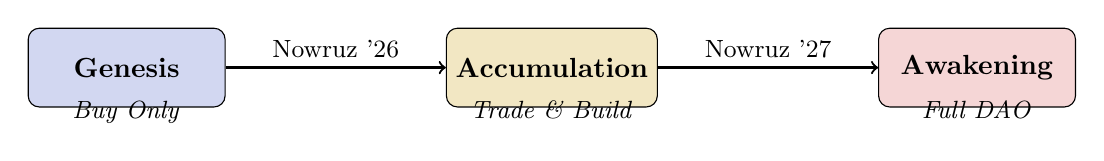
\begin{tikzpicture}[scale=1.2]
    \node[draw, rounded corners, fill=persianblue!20, minimum width=2.5cm, minimum height=1cm] (genesis) at (0,0) {\textbf{Genesis}};
    \node[draw, rounded corners, fill=persiangold!30, minimum width=2.5cm, minimum height=1cm] (accum) at (4.5,0) {\textbf{Accumulation}};
    \node[draw, rounded corners, fill=persianred!20, minimum width=2.5cm, minimum height=1cm] (awaken) at (9,0) {\textbf{Awakening}};

    \draw[->, thick] (genesis) -- (accum) node[midway, above] {\small Nowruz '26};
    \draw[->, thick] (accum) -- (awaken) node[midway, above] {\small Nowruz '27};

    \node[below=0.3cm] at (genesis) {\small\textit{Buy Only}};
    \node[below=0.3cm] at (accum) {\small\textit{Trade \& Build}};
    \node[below=0.3cm] at (awaken) {\small\textit{Full DAO}};
\end{tikzpicture}
\end{center}

This deliberate, patient approach demonstrates our commitment to building something lasting --- not a pump-and-dump scheme, but a genuine movement to unite the Persian diaspora and honor Cyrus the Great's legacy.

\section{The Vision: A Free Iran}

\subsection{What We Are Building Toward}

We are not building a cryptocurrency project. We are building the infrastructure for Iranian liberation and reconstruction. When the Islamic Republic falls---and it \textit{will} fall---we will be ready.

\begin{tcolorbox}[colback=persiangold!10!white,colframe=persianblue,width=\textwidth,arc=3mm,boxrule=2pt]
\centering
\textbf{\Large The Iran We Will Build}

\vspace{0.3cm}

\begin{tabular}{ll}
\textbf{Secular} & Religion is personal, government is for all\\
\textbf{Democratic} & Chosen by the people, accountable to the people\\
\textbf{Federal} & Respecting all ethnicities and regions\\
\textbf{Modern} & Leading in technology, science, culture\\
\textbf{Prosperous} & An economy worthy of our human capital\\
\textbf{Free} & The Cyrus Cylinder as our constitution\\
\end{tabular}
\end{tcolorbox}

\subsection{The DAO's Role in Liberation}

The CYRUS DAO treasury will fund direct action for Iranian freedom:

\textbf{Immediate Priorities:}
\begin{itemize}[leftmargin=*]
    \item \textbf{Secure Communications} --- Fund VPN and encryption tools for activists inside Iran
    \item \textbf{Protest Support} --- Legal defense, medical aid, family support for arrested protesters
    \item \textbf{Media Operations} --- Independent Persian journalism, documentary production
    \item \textbf{International Advocacy} --- Lobbying democratic governments for support
    \item \textbf{Activist Networks} --- Connecting cells inside Iran with diaspora resources
\end{itemize}

\textbf{Transition Phase (When the Regime Falls):}
\begin{itemize}[leftmargin=*]
    \item \textbf{Interim Government Support} --- Technical expertise for transition administration
    \item \textbf{Election Infrastructure} --- Transparent voting systems for first free elections
    \item \textbf{Security Sector Reform} --- Training for democratic policing
    \item \textbf{Media Pluralism} --- Funding independent newspapers, TV, radio
    \item \textbf{Civil Society} --- Grants for NGOs, unions, professional associations
\end{itemize}

\textbf{Reconstruction Phase:}
\begin{itemize}[leftmargin=*]
    \item \textbf{Schools} --- Rebuild secular education from primary to university
    \item \textbf{Healthcare} --- Modern hospitals, clinics, medical training
    \item \textbf{Infrastructure} --- Roads, bridges, telecommunications
    \item \textbf{Environment} --- Restore Lake Urmia, forests, air quality
    \item \textbf{Cultural Sites} --- Preserve Persepolis, Pasargadae, Isfahan
    \item \textbf{Repatriation Support} --- Help diaspora families return home
\end{itemize}

\subsection{A Call to Every Persian}

This is bigger than any token, any investment, any individual. This is about:

\begin{center}
\textit{Your grandmother who still dreams of the Iran of her youth.}\\
\textit{Your cousins who cannot speak freely in their own country.}\\
\textit{The young woman who removed her hijab and was beaten for it.}\\
\textit{The student who tweeted and was imprisoned for it.}\\
\textit{The poet whose words are banned from bookstores.}\\
\textit{The 2,500 years of civilization that refuse to be erased.}
\end{center}

Every CYRUS token you hold is a vote for freedom. Every proposal you support is a brick in the foundation of a new Iran. Every Persian you bring into this community strengthens our collective power.

\begin{tcolorbox}[colback=persianred!10!white,colframe=persianred,width=\textwidth,arc=3mm,boxrule=2pt]
\centering
\textbf{\Large M\=a Ham\=e B\=a Ham Hast\=im}\\
\vspace{0.2cm}
\textit{We Are All Together}\\
\vspace{0.3cm}
The regime divides us by ethnicity, by religion, by politics.\\
\textbf{CYRUS unites us by heritage, by values, by destiny.}\\
\vspace{0.2cm}
Persian, Kurd, Azeri, Baluch, Lor, Gilaki, Arab---\\
\textbf{We are all children of Cyrus. We are all Iran.}
\end{tcolorbox}

\newpage

\section{Liberation Infrastructure: Theory \& Design}

\begin{center}
\textit{We were scattered like dust in the wind---\\
then we remembered we are one fire.\\
Not to burn the world---\\
to light a path home.}
\end{center}

\vspace{0.5cm}

This section grounds our mission in political philosophy and institutional design. Freedom is not vibes---it is engineering. The following framework synthesizes classical political theory with modern mechanism design to explain \textit{why} decentralized, transparent institutions outcompete authoritarian alternatives, and \textit{how} CYRUS instantiates these principles.

\subsection{Political Foundations: Why Free Republics Prevail}

\subsubsection{Rousseau: Legitimacy Requires Consent}

Jean-Jacques Rousseau's core insight remains foundational: political authority is legitimate only if it arises from a contract among equals, oriented toward the common interest rather than the ruler's interest. The ``general will'' is not mob mood---it is the institutionalized expression of the common good under rules that apply equally to all.

\textbf{CYRUS Application:}
\begin{itemize}[leftmargin=*]
    \item A community treasury is only ``ours'' if the rules of spending are consented to, auditable, and amendable by the governed
    \item Freedom is not sentiment; it is rule-bound self-government
    \item DAO governance implements Rousseau's vision: transparent rules, equal standing, institutions that convert collective preferences into binding decisions without privileging any caste, clerical class, or faction
\end{itemize}

\subsubsection{Montesquieu: Tyranny as Systems Failure}

Charles de Montesquieu's insight cuts deeper than ``bad leaders.'' Tyranny is what happens when legislative, executive, and judicial power collapse into one hand. The remedy is structural---separation of powers plus checks and balances.

\textbf{CYRUS Application:}
\begin{itemize}[leftmargin=*]
    \item A DAO is not automatically democratic
    \item It must be designed so that proposers cannot instantly execute
    \item Execution must be constrained (timelock + multisig)
    \item Constitutional changes require supermajorities
    \item Power is distributed, slowed, and made reversible
\end{itemize}

\begin{tcolorbox}[colback=persianblue!5!white,colframe=persianblue,width=\textwidth,arc=2mm,boxrule=1pt]
\centering
\textbf{Montesquieu's Principle:}\\
\vspace{0.2cm}
\textit{``When the same actor controls rule-making, enforcement, and adjudication,\\despotism becomes a default. A free republic is therefore an engineering problem:\\distribute power, slow it down, and make it reversible.''}
\end{tcolorbox}

\subsubsection{Marx: Centralized Power Becomes Class Power}

Karl Marx's durable critique warns that centralized institutions tend to become instruments of a ruling class, even when they claim sacred legitimacy. Whether ``class'' is defined by money, party membership, or clerical hierarchy, the pattern holds: centralization $\rightarrow$ capture $\rightarrow$ coercion.

\textbf{CYRUS Application:}
\begin{itemize}[leftmargin=*]
    \item The point is not to ``install Marxism''
    \item The point is to take the warning seriously: \textit{any concentrated power will be captured}
    \item Design must assume capture attempts are constant
    \item Decentralization is not ideology---it is defensive engineering
\end{itemize}

\subsection{Why Democracy Outcompetes Authoritarianism}

\subsubsection{The Democracy Dividend: Growth \& Innovation}

Empirical research demonstrates that democracy causally increases long-run economic performance through education, broader opportunity, accountability, and lower extractive risk.

\begin{itemize}[leftmargin=*]
    \item Authoritarian systems can spike growth briefly via coercion
    \item But innovative, resilient prosperity is more compatible with open institutions, predictable law, and broad participation
    \item Iran's brain drain---millions of educated Persians building other nations' economies---is direct evidence of authoritarian waste
\end{itemize}

\subsubsection{Women's Rights as Macroeconomic Capacity}

If half your population is legally constrained, your economy is constrained. Modern research repeatedly quantifies large welfare losses from gender inequality.

\begin{tcolorbox}[colback=persiangold!10!white,colframe=persiangold,width=\textwidth,arc=2mm,boxrule=1pt]
\centering
\textbf{Women's equality is not only moral---it is state capacity:}\\
\vspace{0.2cm}
Productivity $\bullet$ Entrepreneurship $\bullet$ Legitimacy $\bullet$ Social Stability
\end{tcolorbox}

The Islamic Republic's systematic oppression of women is not just a human rights violation---it is economic self-sabotage. A free Iran with full gender equality would unlock trillions in human potential.

\subsection{Why Blockchain Belongs in Liberation (Without Magic Thinking)}

\subsubsection{What Blockchains Actually Add}

\begin{itemize}[leftmargin=*]
    \item \textbf{Credible Neutrality}: Rules execute the same way for insiders and outsiders
    \item \textbf{Auditability}: Treasury flows are inspectable by anyone, anywhere
    \item \textbf{Composability}: Grants, identity, voting, budgeting become reusable primitives
    \item \textbf{Diaspora Coordination}: Pooled funding and governance across borders, beyond any single jurisdiction
    \item \textbf{Censorship Resistance}: No central authority can freeze accounts or block participation
\end{itemize}

\subsubsection{What Blockchains Do Not Add}

\begin{itemize}[leftmargin=*]
    \item They do not guarantee democracy
    \item They do not prevent oligarchy unless you design against it
    \item They do not make illegal activity acceptable
\end{itemize}

\begin{tcolorbox}[colback=persianblue!10!white,colframe=persianblue,width=\textwidth,arc=2mm,boxrule=1pt]
\centering
\textbf{CYRUS is infrastructure for lawful civic coordination:}\\
\vspace{0.2cm}
Transparent Funding $\bullet$ Community Governance $\bullet$ Durable Institutions
\end{tcolorbox}

\subsection{Constitutional Design: A Three-Branch DAO}

Following Montesquieu, the CYRUS DAO implements separation of powers on-chain:

\begin{table}[h]
\centering
\begin{tabular}{@{}lll@{}}
\toprule
\textbf{Branch} & \textbf{Function} & \textbf{Mechanism} \\ \midrule
Legislative & Deliberation + Voting & Token-weighted proposals \\
Executive & Operations + Implementation & Multisig execution \\
Judicial & Constitutional Review & Dispute resolution \\ \bottomrule
\end{tabular}
\caption{Three-Branch DAO Architecture}
\end{table}

\textbf{Anti-Capture Mechanisms:}
\begin{itemize}[leftmargin=*]
    \item \textbf{Timelock}: 48-hour delay between approval and execution
    \item \textbf{Diverse Multisig}: Multiple signers with geographic and professional diversity, rotating terms
    \item \textbf{Constitution File}: Enumerated rights + spending constraints + amendment procedures
    \item \textbf{Supermajority Thresholds}: Constitutional changes require 67\%+ approval with 20\%+ quorum
    \item \textbf{Veto Period}: Community can block execution during timelock window
\end{itemize}

\subsection{Mathematical Models: Quantifying Freedom}

\subsubsection{Tyranny Risk as a Function of Power Concentration}

Let $C \in [0,1]$ be a concentration index where $1$ represents fully centralized power. We model capture risk as:

\begin{equation}
R_{\text{capture}}(C) = 1 - \exp(-\alpha C^\beta), \qquad \alpha > 0,\ \beta > 1
\end{equation}

\textbf{Interpretation}: Once concentration rises, risk accelerates nonlinearly. This is the mathematical argument for separation of powers, timelocks, and transparency. Small increases in concentration near the top produce dramatic increases in capture risk.

\begin{figure}[h]
\centering
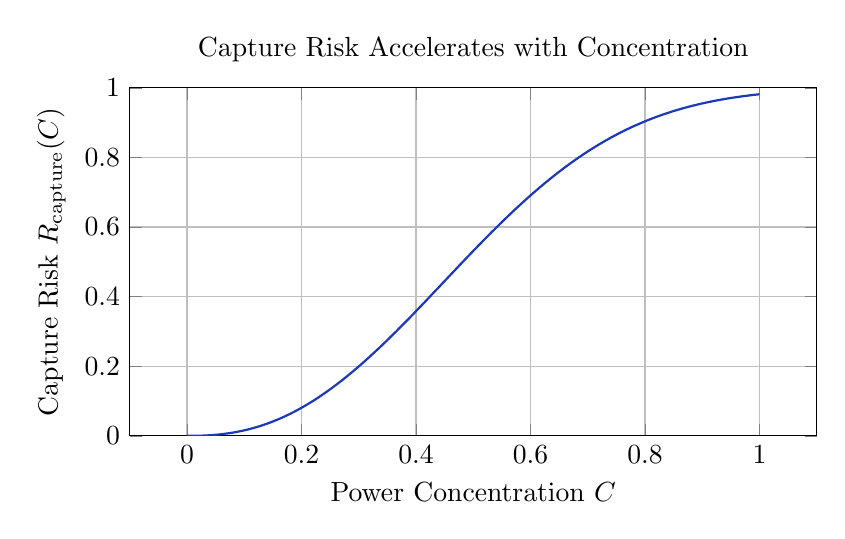
\begin{tikzpicture}
\begin{axis}[
  width=0.85\linewidth, height=6cm,
  xlabel={Power Concentration $C$},
  ylabel={Capture Risk $R_{\text{capture}}(C)$},
  domain=0:1, samples=200,
  ymin=0, ymax=1, grid=both,
  title={Capture Risk Accelerates with Concentration}
]
\addplot[thick, color=persianblue] {1 - exp(-4*x^2.4)};
\end{axis}
\end{tikzpicture}
\caption{Capture risk accelerates nonlinearly as power concentrates. Design must keep $C$ low.}
\end{figure}

\subsubsection{Legitimacy as a Function of Participation and Fairness}

Let $p$ be participation rate and $q$ be perceived fairness (auditability, equal rules). A legitimacy index:

\begin{equation}
L(p, q) = 1 - \exp(-\lambda \cdot p \cdot q), \qquad \lambda > 0
\end{equation}

\textbf{Interpretation}: High legitimacy requires \textit{both} participation and fair process. Neither alone suffices. A 50\% participation rate with 80\% perceived fairness yields higher legitimacy than 80\% participation with rigged rules.

\begin{figure}[h]
\centering
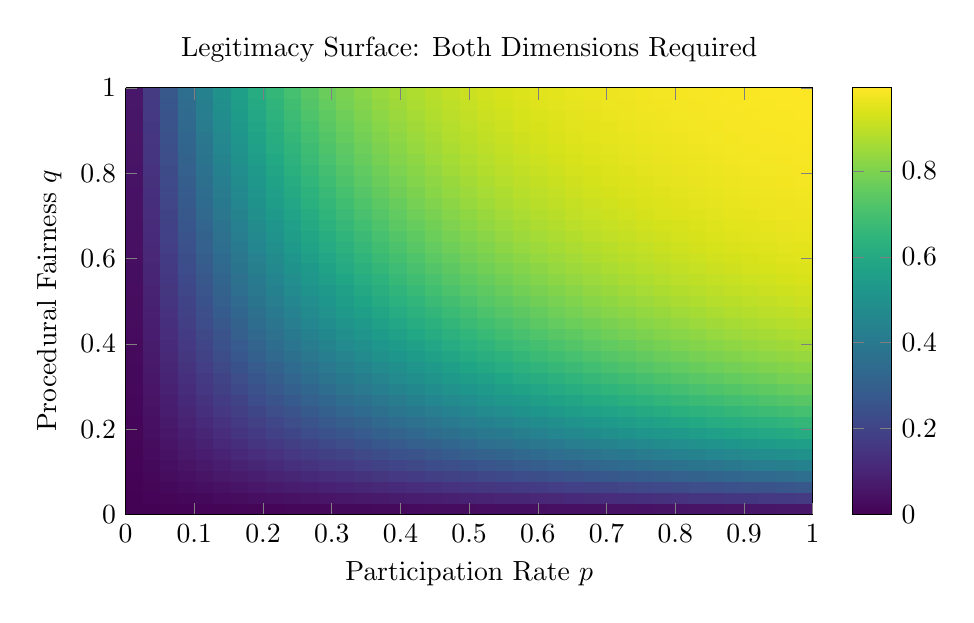
\begin{tikzpicture}
\begin{axis}[
  view={0}{90},
  width=0.85\linewidth, height=7cm,
  xlabel={Participation Rate $p$},
  ylabel={Procedural Fairness $q$},
  colorbar,
  colormap/viridis,
  title={Legitimacy Surface: Both Dimensions Required}
]
\addplot3[
  surf, shader=flat,
  domain=0:1, y domain=0:1,
  samples=40, samples y=40
] {1 - exp(-5*x*y)};
\end{axis}
\end{tikzpicture}
\caption{Legitimacy rises when both participation and procedural fairness are high.}
\end{figure}

\subsubsection{Present Value of a Free Iran}

We cannot price 2,500 years of civilization directly. But we can model the economic value of freedom using present value mathematics.

Let $Y_t$ be annual ``cultural + economic surplus'' attributable to freedom and prosperity, with discount rate $r$:

\begin{equation}
PV = \sum_{t=1}^{T} \frac{Y_t}{(1+r)^t}
\end{equation}

For long-horizon approximation with growth rate $g$ where $r > g$:

\begin{equation}
PV_{\infty} \approx \frac{Y_1}{r - g}
\end{equation}

\textbf{Example}: If a free Iran generates \$100B additional annual surplus over the status quo, with $r = 8\%$ and $g = 3\%$:

\[
PV_{\infty} \approx \frac{\$100B}{0.08 - 0.03} = \$2 \text{ trillion}
\]

This is not speculation---it is the standard approach to valuing long-duration assets.

\subsubsection{Token Value from Captured Share}

For transparency, we present the valuation identity that underlies any rational token pricing:

\begin{equation}
\text{Implied Price} \approx \frac{PV \cdot s \cdot m}{S}
\end{equation}

Where:
\begin{itemize}[leftmargin=*]
    \item $PV$ = Present value of the addressable ``free Iran / diaspora coordination'' economy
    \item $s$ = Capture share (fraction of that economy CYRUS can coordinate)
    \item $m$ = Value accrual fraction (what portion flows to tokenholders via governance, grants, utility)
    \item $S$ = Circulating token supply
\end{itemize}

\begin{figure}[h]
\centering
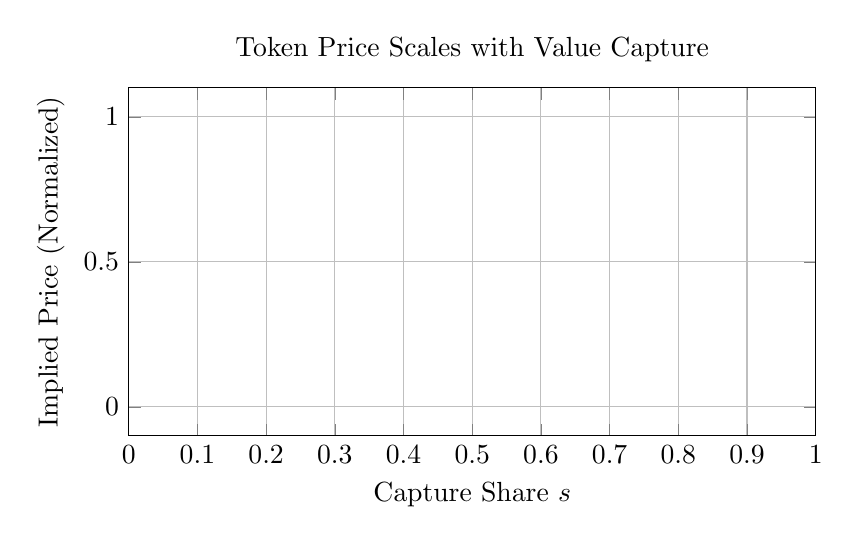
\begin{tikzpicture}
\begin{axis}[
  width=0.85\linewidth, height=6cm,
  xlabel={Capture Share $s$},
  ylabel={Implied Price (Normalized)},
  xmin=0, xmax=0.05,
  grid=both,
  legend pos=north west,
  title={Token Price Scales with Value Capture}
]
\addplot[thick, color=persianblue] {x}; \addlegendentry{$PV \cdot m / S = 1$}
\addplot[thick, color=persiangold] {3*x}; \addlegendentry{$PV \cdot m / S = 3$}
\addplot[thick, color=persianred] {10*x}; \addlegendentry{$PV \cdot m / S = 10$}
\end{axis}
\end{tikzpicture}
\caption{Price scales linearly with capture share; slope depends on value-accrual design.}
\end{figure}

\textbf{Critical Note}: The whitepaper is explicit that $m$ depends on actual mechanisms---governance rights, treasury access, membership utility. Without concrete value accrual, $m \approx 0$ and token value is purely speculative. CYRUS designs for real utility through DAO governance and grant access.

\subsection{How Freedom Wins: The Engineering Summary}

Democracies win sustainably when they:

\begin{enumerate}[leftmargin=*]
    \item \textbf{Reduce the premium on fear}: Rule of law, rights protections, predictable governance make cooperation more attractive than coercion
    \item \textbf{Increase the return to talent}: Education, women's equality, open markets ensure that human capital is developed and deployed efficiently
    \item \textbf{Prevent capture through design}: Checks, transparency, decentralization, and rotation make it structurally difficult for any faction to seize permanent control
\end{enumerate}

This is the engineering lesson of constitutionalism (Montesquieu), legitimacy (Rousseau), and the critique of concentrated power (Marx).

\subsection{The Velvet Path: Nonviolent Transition}

\begin{center}
\textit{``Out beyond ideas of wrongdoing and rightdoing,\\
there is a field. I'll meet you there.\\
When the soul lies down in that grass,\\
the world is too full to talk about.''}\\
\vspace{0.2cm}
--- Rumi
\end{center}

\vspace{0.5cm}

The CYRUS community commits to the \textbf{velvet path}---liberation through legitimacy collapse, not through violence. This is not weakness; it is strategic wisdom rooted in Persian civilization's deepest values.

\subsubsection{Why Nonviolence Wins}

History teaches that violent revolutions often replace one tyranny with another. The French Revolution gave way to the Terror, then Napoleon. The Russian Revolution produced Stalin. The Iranian Revolution of 1979 replaced a flawed monarchy with a theocratic nightmare.

\textbf{Nonviolent transitions, by contrast, build lasting democracies:}
\begin{itemize}[leftmargin=*]
    \item \textbf{Czechoslovakia's Velvet Revolution (1989)}: Peaceful protests, civil disobedience, and moral witness brought down communism without a shot
    \item \textbf{Poland's Solidarity Movement}: Workers, intellectuals, and the Church created parallel institutions that made the regime irrelevant
    \item \textbf{South Africa's Transition}: Despite immense provocation, the ANC chose negotiation and truth-and-reconciliation over vengeance
    \item \textbf{India's Independence}: Gandhi's satyagraha (truth-force) defeated the British Empire through moral authority
\end{itemize}

The pattern is clear: \textit{regimes fall when they lose legitimacy, not when they lose battles.}

\subsubsection{The Persian Way: Cyrus as Model}

Cyrus the Great conquered Babylon without a battle. The gates opened because his reputation preceded him---a reputation for mercy, for honoring local customs, for freeing the enslaved rather than creating new slaves.

\begin{tcolorbox}[colback=persiangold!10!white,colframe=cyruscolor,width=\textwidth,arc=2mm,boxrule=1pt]
\centering
\textbf{Cyrus conquered through legitimacy, not terror.}\\
\vspace{0.2cm}
\textit{The Babylonians welcomed him because he offered something better.\\
This is the model for Iran's liberation: become so obviously better\\
that the regime collapses under the weight of its own illegitimacy.}
\end{tcolorbox}

\subsubsection{How the Diaspora Accelerates Legitimacy Collapse}

The CYRUS DAO contributes to nonviolent regime change by:

\begin{enumerate}[leftmargin=*]
    \item \textbf{Demonstrating Competence}: A well-governed, transparent, effective diaspora institution proves Iranians can self-govern democratically
    \item \textbf{Building Parallel Institutions}: Cultural organizations, educational programs, humanitarian networks that serve Iranians regardless of the regime
    \item \textbf{Documenting Truth}: Funding journalism, human rights documentation, and historical preservation that expose the regime's crimes
    \item \textbf{Maintaining Hope}: Every grant for a Persian language school, every scholarship, every cultural event tells Iranians: \textit{we are building the future}
    \item \textbf{Preparing Transition}: Training administrators, lawyers, educators, and civil servants who will staff a democratic Iran
\end{enumerate}

\textbf{We do not seek to destroy the regime. We seek to make it irrelevant.}

\subsection{Reconciliation, Not Revenge}

\begin{center}
\textit{``If you are irritated by every rub,\\
how will you be polished?''}\\
\vspace{0.2cm}
--- Rumi
\end{center}

\vspace{0.5cm}

When freedom comes---and it \textit{will} come---we face a choice that will define Iran for generations: revenge or reconciliation.

The CYRUS community chooses reconciliation.

\subsubsection{The Poison of Vengeance}

After 1979, the new regime executed thousands. Families were destroyed. Communities were shattered. The cycle of violence that began then continues today---protesters shot, activists hanged, children killed.

If we respond to violence with violence, we perpetuate the cycle. We become what we sought to replace.

\subsubsection{The South African Model}

When apartheid fell, South Africa faced the same choice. Nelson Mandela and Desmond Tutu chose the Truth and Reconciliation Commission---not amnesty without accountability, but a process where perpetrators could confess their crimes in exchange for the truth being heard.

\textbf{Iran will need something similar:}
\begin{itemize}[leftmargin=*]
    \item \textbf{Truth}: Full documentation of crimes---executions, torture, corruption, theft
    \item \textbf{Acknowledgment}: Public recognition of what was done and to whom
    \item \textbf{Accountability}: Those who gave orders face justice; those who followed orders under duress may qualify for amnesty if they confess fully
    \item \textbf{Restitution}: Stolen assets returned; victims' families compensated
    \item \textbf{Healing}: National programs to process collective trauma
\end{itemize}

\subsubsection{Who Is Our Enemy?}

\begin{tcolorbox}[colback=persianblue!10!white,colframe=persianblue,width=\textwidth,arc=3mm,boxrule=2pt]
\centering
\textbf{\Large Our enemy is not the Iranian people who served the regime.}\\
\vspace{0.3cm}
Our enemy is the \textit{system}---the structures of oppression, the mechanisms of control,\\
the ideology that crushes human dignity.\\
\vspace{0.2cm}
Many who work within the system do so to survive, to protect their families,\\
to carve out small spaces of decency within an indecent structure.\\
\vspace{0.2cm}
\textbf{When freedom comes, we will need them to help rebuild.}
\end{tcolorbox}

The revolutionary guards who defect, the bureaucrats who preserve records, the judges who quietly reduce sentences, the teachers who smuggle forbidden ideas into classrooms---these are not our enemies. They are Iranians trapped in an unjust system, waiting for the chance to do better.

\subsubsection{The Example of Reza Pahlavi}

Crown Prince Reza Pahlavi has consistently called for reconciliation rather than revenge. He has:
\begin{itemize}[leftmargin=*]
    \item Refused to demonize ordinary Iranians who work within the system
    \item Called for an inclusive transition that welcomes all Iranians
    \item Emphasized that he seeks no throne---only Iran's freedom
    \item Modeled dignity and restraint despite having every reason for bitterness
\end{itemize}

This is the Cyrus legacy: \textit{mercy to the defeated, welcome to the convert, justice tempered with wisdom.}

\subsection{The Romantic Vision: What a Free Iran Looks Like}

\begin{center}
\textit{``I have lived on the lip of insanity,\\
wanting to know reasons,\\
knocking on a door. It opens.\\
I've been knocking from the inside.''}\\
\vspace{0.2cm}
--- Rumi
\end{center}

\vspace{0.5cm}

Let us paint the picture. Not as fantasy, but as vision---the Iran we are building toward, the Iran that awaits on the other side of this struggle.

\subsubsection{The Return of Persian Culture}

Imagine Tehran in spring. The Alborz mountains still snow-capped, the city blooming with cherry blossoms. But now:

\begin{itemize}[leftmargin=*]
    \item \textbf{Music fills the streets}: The tar and setar, the santur and kamancheh, the voices of singers no longer forbidden. Concerts in Azadi Square. Jazz clubs in Darband. Opera at Vahdat Hall.
    \item \textbf{Women walk freely}: Hair in the wind, faces to the sun. Fashion boutiques on Valiasr. Women CEOs, women judges, women ministers. A woman president, perhaps.
    \item \textbf{Artists create without fear}: Filmmakers telling true stories. Poets publishing without censors. Painters exhibiting without permission. Tehran as the cultural capital of the Middle East once more.
    \item \textbf{Young people dance}: In clubs, at weddings, in the streets during Nowruz. The joy that is every Iranian's birthright, restored.
\end{itemize}

\subsubsection{The Healing of the Land}

Iran's environment has been devastated by mismanagement. A free Iran will:

\begin{itemize}[leftmargin=*]
    \item \textbf{Restore Lake Urmia}: Once the largest lake in the Middle East, now a salt flat. With proper management, it can live again.
    \item \textbf{Replant the forests}: The Hyrcanian forests, older than the ice age, protected and expanded. The Zagros reforested.
    \item \textbf{Clean the air}: Tehran's smog replaced with the clear mountain air that once defined the city.
    \item \textbf{Protect the cheetahs}: The Asiatic cheetah, Iran's national animal, saved from extinction. Persian fallow deer roaming free.
\end{itemize}

\subsubsection{The Return of the Diaspora}

Eight million Iranians live abroad. Many dream of return. A free Iran means:

\begin{itemize}[leftmargin=*]
    \item \textbf{Grandchildren meeting grandparents}: Families reunited after decades of separation
    \item \textbf{Skills coming home}: Engineers, doctors, scientists, entrepreneurs bringing expertise built abroad
    \item \textbf{Investment flowing in}: Diaspora capital rebuilding infrastructure, starting businesses, creating jobs
    \item \textbf{Dual lives}: Some will return permanently. Others will split time. All will finally have the \textit{choice}.
\end{itemize}

\subsubsection{Iran Among Nations}

A free, democratic Iran transforms the region:

\begin{itemize}[leftmargin=*]
    \item \textbf{Peace with neighbors}: No more funding of proxy wars. Normal relations with Arab states, Israel, the West.
    \item \textbf{Economic integration}: Iran's oil and gas, but also tech, tourism, agriculture. The Silk Road reborn.
    \item \textbf{Cultural leadership}: Persian language, art, and philosophy inspiring the world as they did for millennia.
    \item \textbf{Moral authority}: A nation that freed itself nonviolently, reconciled with its past, and built a just future. A model for others.
\end{itemize}

\subsection{A Love Letter to Iran}

\begin{center}
\textit{``Let the beauty we love be what we do.\\
There are hundreds of ways to kneel and kiss the ground.''}\\
\vspace{0.2cm}
--- Rumi
\end{center}

\vspace{0.5cm}

To Iran---

You are not the regime that occupies you.

You are the mountains and the deserts, the Caspian shores and the Persian Gulf. You are Persepolis and Pasargadae, Isfahan and Shiraz. You are the poetry of Hafez and Rumi, the mathematics of Khayyam, the medicine of Avicenna.

You are the grandmother who still makes tahdig perfectly. The grandfather who recites Shahnameh from memory. The mother who teaches her daughter to read despite the morality police. The father who dreams of a better future for his sons.

You are the young woman who removed her hijab and walked into history. The student who tweeted and went to prison. The worker who struck. The artist who painted forbidden dreams. The musician who played forbidden songs.

You are 85 million people carrying 2,500 years of civilization in your hearts.

\textbf{You are not defeated. You are not forgotten. You are not alone.}

We, your children scattered across the earth, hold you in our hearts. We build this token, this DAO, this movement---not for profit, not for power---but for \textit{you}.

Every CYRUS token is a vote for your freedom.\\
Every proposal passed is a brick in your future.\\
Every grant given is a seed planted in your soil.

We will not rest until you are free.

We will not rest until your daughters walk in sunlight.\\
Until your sons sing without fear.\\
Until your poets write without censors.\\
Until your scientists discover without limits.\\
Until your lovers love without hiding.

\textit{M\=a ham\=e b\=a ham hast\=im.}\\
We are all together.

\textit{Zendeh b\=ad Ir\=an.}\\
Long live Iran.

\begin{tcolorbox}[colback=persiangold!10!white,colframe=persianblue,width=\textwidth,arc=3mm,boxrule=2pt]
\centering
\textbf{\Large The CYRUS Thesis}

\vspace{0.3cm}

A transparent, decentralized, constitutionally constrained DAO---\\
governed by the Persian diaspora, funded by the bonding curve,\\
and oriented toward liberation and reconstruction---\\
is a \textit{structurally superior} institution for achieving freedom\\
compared to any centralized alternative.

\vspace{0.3cm}

\textit{This is not hope. This is design.}
\end{tcolorbox}

\section{Join the Movement}

\subsection{For the Persian Diaspora}

CYRUS is more than a token---it's a movement to unite and empower the global Persian community. Whether your family left Iran in 1979 or your ancestors were part of earlier migrations, whether you speak fluent Farsi or are learning your heritage language, whether you live in Tehrangeles or a small town with no other Persians---CYRUS welcomes you.

\textbf{How to Participate:}

\begin{enumerate}[leftmargin=*]
    \item \textbf{Acquire CYRUS}: Purchase through the bonding curve with USDT
    \item \textbf{Join the Community}: Connect with fellow Persians worldwide
    \item \textbf{Participate in Governance}: Vote on proposals, submit ideas
    \item \textbf{Share Your Heritage}: Create content, teach others
    \item \textbf{Support Initiatives}: Contribute to cultural preservation
\end{enumerate}

\subsection{For Friends of Persia}

You don't need Persian blood to appreciate the legacy of Cyrus the Great. His principles---freedom, tolerance, human dignity---belong to all humanity. We welcome anyone who shares these values.

\begin{itemize}[leftmargin=*]
    \item History enthusiasts interested in ancient Persia
    \item Human rights advocates inspired by the Cyrus Cylinder
    \item Cultural preservation supporters
    \item Anyone who believes in the principles Cyrus championed
\end{itemize}

\section{Conclusion: The Spirit of Cyrus Lives On}

Twenty-five centuries have passed since Cyrus the Great conquered Babylon and proclaimed freedom for the enslaved, dignity for the oppressed, and tolerance for all beliefs. Empires have risen and fallen. The world has transformed beyond recognition. Yet the principles he championed remain as vital as ever.

Today, millions of Persians live scattered across the globe---a diaspora born of upheaval but carrying within it the seeds of a great civilization. We carry the poetry of Rumi and Hafez in our hearts, the mathematics of Khayyam in our minds, and the principles of Cyrus in our souls.

\textbf{But we also carry a burden: the knowledge that our homeland is not free.}

For over forty years, the Iranian people have lived under a regime that betrays everything Cyrus stood for. Where he freed the enslaved, they imprison the innocent. Where he honored all faiths, they impose religious tyranny. Where he celebrated human dignity, they execute dissidents and beat women in the streets.

\textbf{This ends with us.}

The CYRUS token is not just a symbol---it is a tool. A tool for organizing the diaspora. A tool for funding resistance. A tool for building the institutions that a free Iran will need. A tool for turning our collective grief and anger into collective action.

When the historians of the future write the story of Iran's liberation, they will ask: \textit{``Where were you? What did you do?''}

Let our answer be: \textit{``We were there. We organized. We funded. We fought. We won.''}

As it is written at Pasargadae:

\begin{center}
\textit{``O man, whoever you are, from wherever you come,\\
for I know you shall come---\\
I am Cyrus, who founded the Persian Empire.''}
\end{center}

We have come, O Cyrus. We have come from Los Angeles and London, from Toronto and Tel Aviv, from every corner of the world where your children have scattered. We have come with blockchain as our tool and your principles as our guide.

\textbf{And we will not rest until Iran is free.}

\vspace{1cm}

\begin{center}
\rule{0.5\textwidth}{0.4pt}

\vspace{0.5cm}

{\Large\bfseries\color{persianblue} Zendeh B\=ad Kourosh-e Bozorg}

\vspace{0.2cm}

{\large Long Live Cyrus the Great}

\vspace{0.3cm}

{\Large\bfseries\color{persianred} Zendeh B\=ad Ir\=an}

\vspace{0.2cm}

{\large Long Live Iran}

\vspace{0.5cm}

\textbf{\large Zan, Zendegi, \=Az\=adi}

\vspace{0.2cm}

\textit{Woman, Life, Freedom}

\vspace{0.5cm}

{\color{persiangold}$\bigstar$} \textsc{For the PARS Community \& Diaspora} {\color{persiangold}$\bigstar$}

\vspace{0.3cm}

{\color{persiangold}$\bigstar$} \textsc{For a Free Iran} {\color{persiangold}$\bigstar$}

\end{center}

\newpage

\section{The Path to Universal Liberty}

\begin{center}
\textit{``The wound is the place where the Light enters you.''}\\
\vspace{0.2cm}
--- Rumi
\end{center}

\vspace{0.5cm}

The struggle for Iranian freedom is part of a larger story---the story of humanity's long march toward liberty. From the Cyrus Cylinder to the Magna Carta, from the Declaration of the Rights of Man to the Universal Declaration of Human Rights, from Gandhi's salt march to Mandela's long walk to freedom---we stand in a tradition of those who dared to imagine a world where every person lives in dignity.

\subsection{Freedom as a Universal Principle}

Cyrus the Great did not liberate only Persians. He freed Babylonians, Jews, Elamites, Medes---every people under his rule. His principle was universal: \textit{all human beings deserve freedom and dignity, regardless of their origin, faith, or station.}

This universalism is our inheritance and our obligation.

\begin{tcolorbox}[colback=persianblue!10!white,colframe=persianblue,width=\textwidth,arc=3mm,boxrule=2pt]
\centering
\textbf{\Large The CYRUS Principles of Universal Liberty}

\vspace{0.3cm}

\begin{enumerate}[leftmargin=*]
    \item \textbf{Dignity is inherent}: Every human being possesses inviolable dignity by virtue of being human
    \item \textbf{Freedom is indivisible}: No one is truly free until all are free
    \item \textbf{Power must be accountable}: Authority derives from consent and serves the governed
    \item \textbf{Truth must be spoken}: Transparency and honest witness are moral imperatives
    \item \textbf{Mercy transcends vengeance}: Justice seeks healing, not destruction
    \item \textbf{The future belongs to builders}: Those who create outcompete those who destroy
\end{enumerate}
\end{tcolorbox}

\subsection{The Tools of Liberation}

Every liberation movement requires tools. Ours include:

\begin{itemize}[leftmargin=*]
    \item \textbf{Economic coordination}: The CYRUS token and DAO treasury
    \item \textbf{Transparent governance}: On-chain voting and constitutional constraints
    \item \textbf{Cultural preservation}: Funding for language, art, heritage
    \item \textbf{Humanitarian action}: Direct support for those in need
    \item \textbf{Secure communications}: Cryptographic protocols that cannot be surveilled
    \item \textbf{Truth documentation}: Journalism, human rights records, historical archives
\end{itemize}

The following section specifies a communications protocol that ensures activists, journalists, and ordinary citizens can coordinate without fear of interception.

\section{CYRUS Protocol: Post-Quantum Secure Communications}

\begin{center}
\textit{``Raise your words, not your voice.\\
It is rain that grows flowers, not thunder.''}\\
\vspace{0.2cm}
--- Rumi
\end{center}

\vspace{0.5cm}

Liberation requires coordination. Coordination requires communication. And communication under surveillance is not communication---it is entrapment.

The CYRUS community recommends and supports the development of post-quantum secure messaging protocols that protect activists, journalists, and citizens from both current surveillance and future quantum attacks. This section specifies the technical requirements and architecture.

\subsection{Threat Model}

We assume adversaries with:
\begin{itemize}[leftmargin=*]
    \item \textbf{Mass surveillance capability}: Ability to intercept and store all network traffic
    \item \textbf{State-level resources}: Access to nation-state cryptanalytic capabilities
    \item \textbf{Future quantum computers}: Ability to break classical asymmetric cryptography (RSA, ECDH) within 10--20 years
    \item \textbf{Endpoint compromise attempts}: Malware, physical seizure, coercion
    \item \textbf{Network-level attacks}: Traffic analysis, timing attacks, node compromise
\end{itemize}

\subsection{Security Goals}

The protocol must achieve:

\begin{table}[h]
\centering
\begin{tabular}{@{}ll@{}}
\toprule
\textbf{Property} & \textbf{Description} \\ \midrule
Confidentiality & Only intended recipients can read messages \\
Authenticity & Recipients can verify sender identity \\
Forward Secrecy & Past messages safe even if keys later compromised \\
Post-Compromise Security & Recovery after temporary key compromise \\
Metadata Protection & Sender/recipient relationship hidden from observers \\
Post-Quantum Resistance & Secure against quantum cryptanalysis \\
Offline Capability & Messages deliverable when recipient offline \\
Multi-Device Support & Seamless use across multiple devices \\
Decentralization & No single point of failure or control \\
\bottomrule
\end{tabular}
\caption{CYRUS Protocol Security Requirements}
\end{table}

\subsection{Cryptographic Primitives}

\subsubsection{Hybrid Post-Quantum Key Exchange}

Classical elliptic curve cryptography (X25519) is efficient but vulnerable to Shor's algorithm on quantum computers. Post-quantum lattice-based schemes (ML-KEM/CRYSTALS-Kyber) resist quantum attacks but are newer and less battle-tested.

\textbf{Solution}: Hybrid key exchange combining both:

\begin{equation}
K_{\text{shared}} = \text{KDF}(K_{\text{X25519}} \| K_{\text{ML-KEM}})
\end{equation}

Security holds unless \textit{both} schemes are broken---classical cryptanalysis defeats ML-KEM \textit{and} quantum computers defeat X25519 simultaneously.

\begin{table}[h]
\centering
\begin{tabular}{@{}lll@{}}
\toprule
\textbf{Primitive} & \textbf{Algorithm} & \textbf{Purpose} \\ \midrule
Classical KEM & X25519 & ECDH key agreement \\
Post-Quantum KEM & ML-KEM-768 (Kyber) & Quantum-resistant key encapsulation \\
Symmetric Encryption & ChaCha20-Poly1305 & AEAD for message encryption \\
Key Derivation & HKDF-SHA256 & Derive session keys from shared secrets \\
Signatures & Ed25519 + Dilithium & Authentication (hybrid PQ) \\
Hash Function & SHA-256/SHA-3 & Integrity, ratchet advancement \\
\bottomrule
\end{tabular}
\caption{Cryptographic Primitives}
\end{table}

\subsubsection{Double Ratchet with PQ Enhancement}

The Double Ratchet algorithm (Signal Protocol) provides forward secrecy and post-compromise security. We enhance it with post-quantum key encapsulation:

\begin{enumerate}[leftmargin=*]
    \item \textbf{Root Key Ratchet}: Updated with each new DH/KEM exchange
    \item \textbf{Sending/Receiving Chains}: Derived from root key, advanced per-message
    \item \textbf{Message Keys}: Ephemeral, deleted immediately after use
    \item \textbf{PQ Ratchet}: Periodic ML-KEM re-keying for quantum resistance
\end{enumerate}

\begin{figure}[h]
\centering
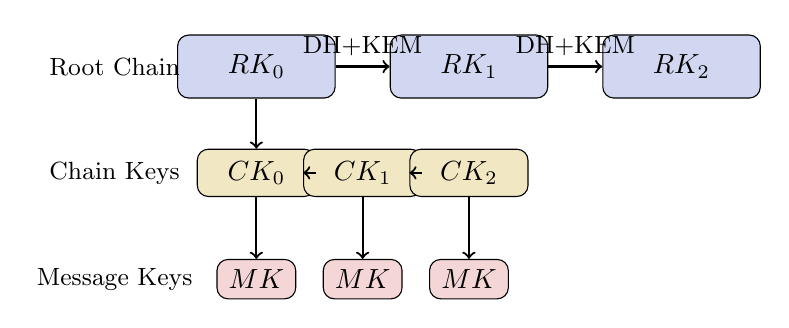
\begin{tikzpicture}[scale=0.9]
    % Root chain
    \node[draw, rounded corners, fill=persianblue!20, minimum width=2cm, minimum height=0.8cm] (rk1) at (0,3) {$RK_0$};
    \node[draw, rounded corners, fill=persianblue!20, minimum width=2cm, minimum height=0.8cm] (rk2) at (3,3) {$RK_1$};
    \node[draw, rounded corners, fill=persianblue!20, minimum width=2cm, minimum height=0.8cm] (rk3) at (6,3) {$RK_2$};

    \draw[->, thick] (rk1) -- (rk2) node[midway, above] {\small DH+KEM};
    \draw[->, thick] (rk2) -- (rk3) node[midway, above] {\small DH+KEM};

    % Sending chains
    \node[draw, rounded corners, fill=persiangold!30, minimum width=1.5cm, minimum height=0.6cm] (ck1) at (0,1.5) {$CK_0$};
    \node[draw, rounded corners, fill=persiangold!30, minimum width=1.5cm, minimum height=0.6cm] (ck2) at (1.5,1.5) {$CK_1$};
    \node[draw, rounded corners, fill=persiangold!30, minimum width=1.5cm, minimum height=0.6cm] (ck3) at (3,1.5) {$CK_2$};

    \draw[->, thick] (rk1) -- (ck1);
    \draw[->, thick] (ck1) -- (ck2);
    \draw[->, thick] (ck2) -- (ck3);

    % Message keys
    \node[draw, rounded corners, fill=persianred!20, minimum width=1cm, minimum height=0.5cm] (mk1) at (0,0) {$MK$};
    \node[draw, rounded corners, fill=persianred!20, minimum width=1cm, minimum height=0.5cm] (mk2) at (1.5,0) {$MK$};
    \node[draw, rounded corners, fill=persianred!20, minimum width=1cm, minimum height=0.5cm] (mk3) at (3,0) {$MK$};

    \draw[->, thick] (ck1) -- (mk1);
    \draw[->, thick] (ck2) -- (mk2);
    \draw[->, thick] (ck3) -- (mk3);

    % Labels
    \node at (-2,3) {\small Root Chain};
    \node at (-2,1.5) {\small Chain Keys};
    \node at (-2,0) {\small Message Keys};
\end{tikzpicture}
\caption{Post-Quantum Enhanced Double Ratchet}
\end{figure}

\subsection{Anonymous Transport: Onion Routing}

Messages are wrapped in multiple encryption layers and routed through a network of nodes, so no single node knows both sender and recipient.

\subsubsection{Three-Hop Onion Requests}

\begin{enumerate}[leftmargin=*]
    \item \textbf{Entry Node}: Knows sender IP, but not destination or content
    \item \textbf{Middle Node}: Knows only previous and next hop
    \item \textbf{Exit Node}: Knows destination swarm, but not sender
\end{enumerate}

Each hop strips one encryption layer:
\begin{equation}
\text{Onion} = E_{K_1}(\text{addr}_2 \| E_{K_2}(\text{addr}_3 \| E_{K_3}(\text{swarm} \| E_{\text{recipient}}(\text{message}))))
\end{equation}

\subsubsection{Decentralized Message Storage (Swarm)}

Messages are stored in recipient's ``swarm''---a set of nodes determined by a DHT (Distributed Hash Table) based on recipient's public key. This enables:
\begin{itemize}[leftmargin=*]
    \item \textbf{Offline delivery}: Messages persist until recipient retrieves them
    \item \textbf{Redundancy}: Multiple nodes store each message
    \item \textbf{Censorship resistance}: No single node can block delivery
    \item \textbf{Expiration}: Messages auto-delete after configurable period
\end{itemize}

\subsection{Multi-Device Architecture}

Users need messaging across phone, laptop, tablet. The protocol supports this via:

\begin{itemize}[leftmargin=*]
    \item \textbf{Per-Account Keys}: Master identity key pair (long-term)
    \item \textbf{Per-Device Keys}: Each device has unique keys linked to account
    \item \textbf{Config Messages}: Encrypted sync of device list, settings, contacts
    \item \textbf{Explicit Device Management}: Users can add/remove devices, revoke compromised ones
\end{itemize}

\subsection{Implementation Recommendations}

The CYRUS community endorses and recommends:

\begin{itemize}[leftmargin=*]
    \item \textbf{Session Messenger}: Open-source, implements this architecture, actively developing Protocol V2 with PQ support
    \item \textbf{Signal Protocol}: Excellent ratchet design, adding PQ (PQXDH)
    \item \textbf{Matrix/Element}: Decentralized, end-to-end encrypted, federation model
\end{itemize}

\textbf{For activists inside Iran}: Use Session or Signal over Tor/VPN. Assume all unencrypted communications are monitored. Delete messages after reading. Use disappearing messages. Never discuss operational details over any electronic medium unless absolutely necessary.

\subsection{The Mathematics of Freedom}

Cryptography is mathematics in service of liberty. The security of these protocols rests on problems believed to be computationally hard:

\begin{itemize}[leftmargin=*]
    \item \textbf{Discrete Logarithm Problem}: Given $g^x \mod p$, find $x$ (classical security)
    \item \textbf{Elliptic Curve DLP}: Given $[k]P$ on curve $E$, find $k$ (compact classical security)
    \item \textbf{Learning With Errors (LWE)}: Given $(\mathbf{A}, \mathbf{As} + \mathbf{e})$, find $\mathbf{s}$ (post-quantum security)
    \item \textbf{Module-LWE}: Structured variant enabling efficient ML-KEM
\end{itemize}

These mathematical structures---groups, rings, lattices---are the foundation of secure communication. Every time an activist sends an encrypted message, they are protected by millennia of mathematical discovery, from Euclid to Diffie-Hellman to the lattice cryptographers of today.

\textbf{This is why we call on mathematicians to join our cause.} Your work is not abstract---it is the armor of the oppressed.

\section{A Call to Artists, Mathematicians, and Cryptographers}

\begin{center}
\textit{``Sell your cleverness and buy bewilderment.\\
Cleverness is mere opinion, bewilderment is intuition.''}\\
\vspace{0.2cm}
--- Rumi
\end{center}

\vspace{0.5cm}

The liberation of Iran---and the broader struggle for human freedom---requires more than activists and organizers. It requires \textit{builders}: those who create the tools, tell the stories, and prove the theorems that make freedom possible.

\subsection{To the Artists}

Persian civilization has always been a civilization of artists. The miniaturists of Isfahan, the poets of Shiraz, the musicians of the classical radif, the filmmakers of the Iranian New Wave---art is how we remember who we are.

\textbf{We need you now.}

\begin{itemize}[leftmargin=*]
    \item \textbf{Visual artists}: Create the imagery of freedom---posters, murals, digital art that inspires and unifies
    \item \textbf{Musicians}: Compose the anthems of liberation---songs that will be sung in the streets of Tehran
    \item \textbf{Writers}: Tell our stories---novels, poems, screenplays that capture the Persian spirit
    \item \textbf{Filmmakers}: Document the struggle---films that bear witness and move hearts
    \item \textbf{Designers}: Build the visual identity of a free Iran---logos, flags, symbols that unite
\end{itemize}

Art is not decoration. Art is \textit{infrastructure}. A movement without art is a movement without soul.

\subsection{To the Mathematicians}

Persian mathematics changed the world. Al-Khwarizmi gave us algebra. Omar Khayyam solved cubic equations. Nasir al-Din Tusi advanced trigonometry. This tradition of rigorous, beautiful mathematics is our heritage.

\textbf{We need your minds.}

\begin{itemize}[leftmargin=*]
    \item \textbf{Cryptographers}: Design and analyze the protocols that protect activists
    \item \textbf{Game theorists}: Model the dynamics of regime collapse and peaceful transition
    \item \textbf{Mechanism designers}: Create voting systems, allocation mechanisms, governance structures that are manipulation-resistant
    \item \textbf{Statisticians}: Analyze human rights data, detect fraud, quantify suffering
    \item \textbf{Complexity theorists}: Prove the hardness assumptions that secure our communications
\end{itemize}

Every theorem you prove, every protocol you design, every attack you discover and fix---these are acts of liberation.

\subsection{To the Cryptographers}

You hold the keys to the kingdom---literally. The protocols you design determine whether activists can coordinate safely, whether journalists can protect sources, whether families can communicate without fear.

\textbf{We need your expertise.}

\begin{itemize}[leftmargin=*]
    \item \textbf{Protocol designers}: Help us build and audit secure communication systems
    \item \textbf{Implementation experts}: Write secure code that withstands real-world attacks
    \item \textbf{Cryptanalysts}: Find vulnerabilities before adversaries do
    \item \textbf{Applied researchers}: Bridge the gap between academic advances and deployed systems
    \item \textbf{Educators}: Teach operational security to activists, journalists, citizens
\end{itemize}

The work you do in your lab, your office, your late-night coding sessions---this work protects lives. This work enables freedom.

\subsection{To the Engineers and Builders}

Software engineers, hardware designers, network architects, systems administrators---you build the infrastructure of the digital world.

\textbf{Build it for freedom.}

\begin{itemize}[leftmargin=*]
    \item \textbf{Contribute to open source}: Session, Signal, Tor, Matrix---these projects need developers
    \item \textbf{Build censorship-circumvention tools}: VPNs, proxies, mesh networks that work inside Iran
    \item \textbf{Design resilient systems}: Decentralized, fault-tolerant, surveillance-resistant
    \item \textbf{Audit and harden}: Find and fix vulnerabilities in freedom tools
    \item \textbf{Document and educate}: Write guides that help non-technical users protect themselves
\end{itemize}

\subsection{The CYRUS Grants for Builders}

The CYRUS DAO will establish grant programs specifically for artists, mathematicians, and engineers working on freedom tools:

\begin{table}[h]
\centering
\begin{tabular}{@{}lll@{}}
\toprule
\textbf{Grant Category} & \textbf{Focus} & \textbf{Examples} \\ \midrule
Art for Freedom & Visual, musical, literary works & Albums, films, murals \\
Cryptographic Research & Protocol design, analysis & New schemes, audits \\
Tool Development & Software for activists & Apps, libraries, guides \\
Education & Training materials & Courses, workshops, docs \\
Documentation & Human rights records & Archives, databases \\
\bottomrule
\end{tabular}
\caption{CYRUS Builder Grants}
\end{table}

\section{News, Updates, and the Living Document}

\begin{center}
\textit{``Yesterday I was clever, so I wanted to change the world.\\
Today I am wise, so I am changing myself.''}\\
\vspace{0.2cm}
--- Rumi
\end{center}

\vspace{0.5cm}

A liberation movement must be adaptive. Conditions change. New challenges emerge. Opportunities arise. The CYRUS ecosystem includes infrastructure for ongoing communication and coordination.

\subsection{Official Channels}

\begin{table}[h]
\centering
\begin{tabular}{@{}lll@{}}
\toprule
\textbf{Channel} & \textbf{Purpose} & \textbf{Update Frequency} \\ \midrule
cyrus.cash & Official website, whitepaper & As needed \\
Twitter/X (@cyrus\_cash) & News, announcements & Daily \\
Telegram (CyrusCommunity) & Community discussion & Real-time \\
Discord & Technical discussion, governance & Real-time \\
GitHub (cyrusdao) & Code, proposals, documentation & Continuous \\
On-chain (Base) & Treasury, governance votes & Per transaction \\
\bottomrule
\end{tabular}
\caption{Official Communication Channels}
\end{table}

\subsection{Governance Proposals as News}

Every DAO proposal is a form of news---a signal of community priorities, a record of decisions, a log of action. The on-chain governance system creates an immutable, transparent record of:

\begin{itemize}[leftmargin=*]
    \item Grant recipients and amounts
    \item Treasury allocations
    \item Constitutional amendments
    \item Community resolutions
\end{itemize}

\subsection{The Whitepaper as Living Document}

This whitepaper is versioned and will be updated as the project evolves. Significant changes require DAO governance approval. The GitHub repository maintains full history:

\begin{center}
\url{https://github.com/cyrusdao/whitepaper}
\end{center}

\textbf{Current Version}: 1.4.0\\
\textbf{Last Updated}: \today

\newpage

\section{Technical Appendix}

\subsection{Smart Contract Specifications}

\begin{table}[h]
\centering
\begin{tabular}{@{}ll@{}}
\toprule
\textbf{Parameter} & \textbf{Value} \\ \midrule
Token Name & Cyrus \\
Token Symbol & CYRUS \\
Token Standard & ERC-20 \\
Decimals & 18 \\
Total Supply & 1,000,000,000 (1 Billion) \\
Blockchain & Base (Coinbase L2) \\
Chain ID & 8453 \\
Payment Token & USDbC (USDT equivalent on Base) \\
USDbC Address & \texttt{0xd9aAEc86B65D86f6A7B5B1b0c42FFA531710b6CA} \\
\bottomrule
\end{tabular}
\caption{Smart Contract Technical Details}
\end{table}

\subsection{Contract Features}

The CYRUS smart contract implements the following security and functionality features:

\begin{itemize}[leftmargin=*]
    \item \textbf{ERC-20 Standard}: Full compatibility with all ERC-20 wallets and exchanges
    \item \textbf{ERC-20 Permit}: Gasless approvals via EIP-2612 signatures
    \item \textbf{ERC-20 Burnable}: Tokens can be burned to reduce supply
    \item \textbf{ERC-20 Pausable}: Emergency pause capability for security
    \item \textbf{Ownable}: Administrative functions protected by ownership
    \item \textbf{ReentrancyGuard}: Protection against reentrancy attacks
    \item \textbf{SafeERC20}: Safe token transfer handling
    \item \textbf{Superchain Bridge}: Compatible with Base/Optimism Superchain bridge
\end{itemize}

\subsection{Transfer Lock Mechanism}

To prevent speculation during the Genesis phase, transfers are locked until Nowruz 2026:

\begin{table}[h]
\centering
\begin{tabular}{@{}ll@{}}
\toprule
\textbf{Parameter} & \textbf{Value} \\ \midrule
Unlock Event & Nowruz 2026 (Spring Equinox) \\
Unlock Date & March 21, 2026 12:00:00 UTC \\
Unix Timestamp & 1742558400 \\
\bottomrule
\end{tabular}
\caption{Transfer Lock Parameters}
\end{table}

\textbf{During Genesis Phase (Before Nowruz 2026):}
\begin{itemize}[leftmargin=*]
    \item Minting (buying from bonding curve) --- \textcolor{green!60!black}{\textbf{Allowed}}
    \item Burning --- \textcolor{green!60!black}{\textbf{Allowed}}
    \item LP wallet transfers (for DEX setup) --- \textcolor{green!60!black}{\textbf{Allowed}}
    \item All other transfers --- \textcolor{red}{\textbf{Blocked}}
\end{itemize}

\textbf{After Nowruz 2026:}
\begin{itemize}[leftmargin=*]
    \item All transfers --- \textcolor{green!60!black}{\textbf{Allowed}}
\end{itemize}

\subsection{Bonding Curve Mathematics}

The quadratic bonding curve is implemented with the following formula:

\begin{equation}
P(s) = P_{start} + (P_{end} - P_{start}) \times \left(\frac{s}{S_{total}}\right)^2
\end{equation}

Where:
\begin{itemize}[leftmargin=*]
    \item $P(s)$ = Price when $s$ tokens have been sold
    \item $P_{start}$ = \$0.01 (10,000 in USDT 6-decimal format)
    \item $P_{end}$ = \$1.00 (1,000,000 in USDT 6-decimal format)
    \item $s$ = Tokens sold so far
    \item $S_{total}$ = 900,000,000 tokens (SALE\_SUPPLY)
\end{itemize}

\textbf{Contract Constants:}
\begin{verbatim}
START_PRICE  = 10000      // $0.01 in USDT (6 decimals)
END_PRICE    = 1000000    // $1.00 in USDT (6 decimals)
SALE_SUPPLY  = 900,000,000 * 10^18  // 900M tokens
LP_RESERVE   = 100,000,000 * 10^18  // 100M tokens
MAX_SUPPLY   = 1,000,000,000 * 10^18 // 1B tokens
\end{verbatim}

\subsection{Security Considerations}

\begin{itemize}[leftmargin=*]
    \item \textbf{Checks-Effects-Interactions}: State updates occur before external calls
    \item \textbf{Slippage Protection}: Optional \texttt{minTokensOut} parameter on buys
    \item \textbf{No Sell Function}: Tokens can only be bought during bonding curve phase
    \item \textbf{Immutable USDT Address}: Payment token address cannot be changed
    \item \textbf{Multi-step Price Calculation}: Accurate integration over quadratic curve
\end{itemize}

\subsection{Contract Functions}

\textbf{Public View Functions:}
\begin{itemize}[leftmargin=*]
    \item \texttt{getCurrentPrice()} --- Returns current price in USDT (6 decimals)
    \item \texttt{calculateTokensForUsdt(amount)} --- Calculate tokens for USDT amount
    \item \texttt{tokensSold()} --- Total tokens sold through bonding curve
    \item \texttt{usdtRaised()} --- Total USDT raised
    \item \texttt{saleActive()} --- Whether bonding curve sale is active
    \item \texttt{transfersEnabled()} --- Whether transfers are unlocked
    \item \texttt{NOWRUZ\_2026()} --- Transfer unlock timestamp
\end{itemize}

\textbf{Public Write Functions:}
\begin{itemize}[leftmargin=*]
    \item \texttt{buy(usdtAmount)} --- Buy tokens with USDT
    \item \texttt{buy(usdtAmount, minTokensOut)} --- Buy with slippage protection
\end{itemize}

\textbf{Owner Functions:}
\begin{itemize}[leftmargin=*]
    \item \texttt{fundLP()} --- Transfer raised USDT to LP wallet
    \item \texttt{setLPWallet(address)} --- Update LP wallet address
    \item \texttt{endSale()} --- End bonding curve sale early
    \item \texttt{resumeSale()} --- Resume paused sale
    \item \texttt{pause()} / \texttt{unpause()} --- Emergency pause controls
\end{itemize}

\subsection{Verified Contract Addresses}

\begin{tcolorbox}[colback=pasargadae!20!white,colframe=cyruscolor,width=\textwidth,arc=2mm,boxrule=1pt]
\textbf{Base Mainnet (Chain ID: 8453)}

\vspace{0.3cm}

CYRUS Token: \texttt{[To be published upon deployment]}

\vspace{0.1cm}

USDbC (Payment): \texttt{0xd9aAEc86B65D86f6A7B5B1b0c42FFA531710b6CA}

\vspace{0.3cm}

\textit{Contract source code will be verified on BaseScan upon deployment.}

\vspace{0.1cm}

\textit{Audit report will be published before launch.}
\end{tcolorbox}

\subsection{Links \& Resources}

\begin{table}[h]
\centering
\begin{tabular}{@{}ll@{}}
\toprule
\textbf{Resource} & \textbf{URL} \\ \midrule
Official Website & \url{https://cyrus.cash} \\
Whitepaper & \url{https://cyrus.cash/whitepaper.pdf} \\
Source Code & \url{https://github.com/luxdao/cyrus} \\
Base Blockchain & \url{https://base.org} \\
BaseScan (Contract) & \url{https://basescan.org/token/[TBD]} \\
DexScreener & \url{https://dexscreener.com/base/[TBD]} \\
Uniswap (Trading) & \url{https://app.uniswap.org} \\
\bottomrule
\end{tabular}
\caption{Official Links (Trading links active after Nowruz 2026)}
\end{table}

\newpage

\section*{DISCLAIMER}
\addcontentsline{toc}{section}{Disclaimer}

\begin{tcolorbox}[colback=persianblue!10!white,colframe=persianblue,width=\textwidth,arc=3mm,boxrule=2pt]

\textbf{\Large THIS IS A COMMUNITY TOKEN}

\vspace{0.3cm}

\textbf{No Financial Advice}: Nothing in this whitepaper constitutes financial, investment, legal, or tax advice. Consult qualified professionals before making any financial decisions.

\vspace{0.2cm}

\textbf{No Expectation of Profit}: CYRUS is a community token honoring Persian heritage and the principles of Cyrus the Great. There is \textbf{NO expectation} of financial gain, profit, or returns of any kind. Token value may go to zero.

\vspace{0.2cm}

\textbf{Assume Total Loss}: Assume any funds used to acquire CYRUS may be lost entirely. Only participate with funds you can afford to lose completely.

\vspace{0.2cm}

\textbf{Community Initiative}: This project is a community initiative created by members of the Persian diaspora. It has no official affiliation with any government, museum, institution, or official entity.

\vspace{0.2cm}

\textbf{Historical Content}: While we strive for historical accuracy, this document is not an academic publication. Consult scholarly sources for detailed historical research.

\vspace{0.2cm}

\textbf{Not a Security}: CYRUS is not a security, investment contract, or financial instrument. It is a community token representing shared cultural values and enabling DAO governance.

\vspace{0.2cm}

\textbf{Regulatory Compliance}: Purchasers are responsible for compliance with local laws and regulations. CYRUS may not be available in all jurisdictions.

\vspace{0.3cm}

\textbf{By acquiring CYRUS tokens, you acknowledge and accept all risks and disclaimers described in this whitepaper.}

\end{tcolorbox}

\vspace{1cm}

\begin{center}
\rule{0.5\textwidth}{0.4pt}

\vspace{0.5cm}

\textbf{Join the PARS Community:}

\vspace{0.3cm}

Website: \url{https://cyrus.cash}

Twitter/X: @cyrus\_cash

Telegram: @CyrusCommunity

Discord: \url{https://discord.gg/cyrus}

GitHub: \url{https://github.com/luxdao/cyrus}

\vspace{0.5cm}

\textit{Honoring the Father of Human Rights}

\vspace{0.2cm}

\textit{Uniting the Persian Diaspora}

\vspace{0.3cm}

{\small Cyrus the Great (Kourosh-e Bozorg) | c. 600--530 BCE}

{\small Founder of the Achaemenid Empire | Author of the Cyrus Cylinder}

\vspace{0.3cm}

{\color{persiangold}$\bigstar$} \textsc{Az M\=a Beh M\=a --- From Us, For Us} {\color{persiangold}$\bigstar$}

\end{center}

\end{document}
